% !TeX program = xelatex
% Generated from the reference PDF text layer; full PDF pages are not embedded.
\PassOptionsToPackage{bookmarks=false}{hyperref}
\documentclass[withoutpreface,bwprint]{cumcmthesis}
\usepackage{url}
\usepackage{subcaption}
\usepackage{graphicx}
\usepackage{svg}
\usepackage{fvextra}
\newfontfamily\PDFTextFont[Path=C:/Windows/Fonts/]{NotoSansSC-Regular.ttf}
\setmonofont{Latin Modern Mono}
\setCJKmonofont[Path=C:/texlive/2025/texmf-dist/fonts/opentype/public/fandol/]{FandolFang-Regular.otf}
\newcommand{\CodeTextSetup}{\xeCJKsetup{CJKecglue={},CJKglue={}}}
\renewcommand{\theFancyVerbLine}{\normalfont\small\arabic{FancyVerbLine}}
\DefineVerbatimEnvironment{CodeText}{Verbatim}{fontsize=\small,numbers=left,numbersep=10pt,xleftmargin=0pt,breaklines=true,breakanywhere=false,breaksymbolleft={},breaksymbolright={},formatcom=\CodeTextSetup,listparameters={\setlength{\topsep}{0pt}\setlength{\partopsep}{0pt}\setlength{\parsep}{0pt}}}
\setlength{\parskip}{0pt}
\sloppy

\makeatletter
\renewenvironment{abstract}{%
\if@twocolumn
    \section*{\abstractname}%
  \else
   \begin{center}%
  {\zihao{4}\bfseries \abstractname\vspace{-.5em}\vspace{\z@}}%
   \end{center}%
   \quotation
  \fi}
  {\if@twocolumn\else\endquotation\clearpage\fi}
\makeatother

\title{基于动态搜索的“板凳龙”运动状态及路线研究}
\tihao{A}
\baominghao{}
\schoolname{}
\membera{}
\memberb{}
\memberc{}
\supervisor{}
\yearinput{2024}
\monthinput{9}
\dayinput{8}

\begin{document}
\maketitle

\begin{abstract}
板凳龙作为浙闽地区的一种传统民俗活动，以其高观赏性和舞龙队的协调配合著称。本文针对板凳龙表演的三个阶段——盘入、调头和盘出，通过分析舞龙队的行进路线及各节板凳之间的几何关系，建立了运动模型和行进路线优化模型。采用多种优化方法，对舞龙队在不同条件下的运动状态以及行进路线进行研究。

\textbf{针对问题一：}构建盘入运动模型。首先，根据盘入路线为等距螺线的特征，建立\textbf{极坐标系}。针对龙头位置，建立有关极角的微分方程，利用微积分及\textbf{二分法}求解龙头前把手的极坐标，继而利用\textbf{余弦定理}，\textbf{递推求解}相邻板凳的位置关系，获得各把手的位置函数。通过对位置函数求导，得到相应的速度函数。最终，将极坐标转换为直角坐标，求得各把手在各时刻的位置和速度，结果详见\textbf{表2，表3和result1.xlsx}。

\textbf{针对问题二：}构建碰撞检测模型。首先，证明最易发生碰撞的区间为最内圈与其外侧一圈的板凳，缩小检测范围。随后，确定\textbf{碰撞条件}为：内圈板凳顶点与外圈板凳把手连线的距离小于板凳宽度的一半（0.15m），并通过几何关系算出\textbf{距离函数}，判断该函数的最小值是否小于0.15m 以确定碰撞是否发生。最后，采用\textbf{动态搜索策略}，先用变步长搜索确定时间范围，再进行二分搜索，确定首次碰撞的准确时间。我们得到停止盘入时间为\textbf{412.473838s}，此时各把手的位置和速度详见\textbf{表4和result2.xlsx}。

\textbf{针对问题三：}构建最短螺距的\textbf{单目标优化}模型。其中目标函数和决策变量为螺距大小。在约束条件方面，基于板凳的几何参数和问题二中的参数限定螺距范围，基于盘入运动模型确定龙头前把手进入调头空间的时间，并利用碰撞检测模型判断进入调头空间前是否发生碰撞，建立相应约束。在优化求解过程中，对比后选用\textbf{粒子群算法}求解板间最小距离，并结合\textbf{变步长搜索}求得最短螺距为\textbf{0.450337m}。

\textbf{针对问题四：}基于问题一的模型，构建调头运动模型。首先证明在给定条件下，调头曲线长度为常数，\textbf{无法进一步减小}。随后，将调头路线划分为四个部分，通过几何关系求解出各部分的曲线方程。沿用问题一的推导方法，首先求解龙头前把手位置函数，再通过递推关系和求导计算其余把手的位置函数和速度函数。我们对调头空间附近的递推进行了详细的\textbf{分类讨论}，并给出了相应的\textbf{递推方程}。最终，将极坐标转换为直角坐标，求得各板凳把手在各时刻的位置和速度，详见\textbf{表5，表6和result4.xlsx}。

\textbf{针对问题五：}在调头运动模型的基础上，构建各把手最大速度的优化模型。首先，通过\textbf{比例转换}，将目标转化为在龙头速度仍为1m/s 的条件下，求解各把手在所有时刻的最大速度。随后，基于问题四的速度规律及物理规律确定最大速度出现的大致时间范围，接着通过大步长搜索确定了最大速度出现的区间为[\textbf{14s},\textbf{15s}]。由于函数在该区间内\textbf{呈单峰性}，应用\textbf{三分搜索算法}进一步精确定位最大速度。最后，通过比例关系还原龙头的最大速度，得到龙头最大速度约为\textbf{1.246266m/s}。

\keywords{板凳龙\quad 等距螺线\quad 动态搜索\quad 粒子群算法\quad 单目标优化}
\end{abstract}

\section{问题重述}
\subsection{问题背景}
中药材在加工后需要及时脱除水分，以提高储藏稳定性并保持成品品质。热风方式利用空气与药材之间的温差和湿度差完成热量、水分交换，药材内部经历由外向内的升温过程，同时水分由内部逐步迁移至表面并逸出。整个过程可分为升温过渡阶段和后续恒温脱水阶段，两个阶段的传热传质特征并不完全相同。

烘房温度、湿度及物性参数的组合会直接影响干燥速率、能耗和最终品质，单纯依靠反复试验难以系统考察这些因素的作用。为此，本文从连续介质传热与传质角度描述药材内部状态的时空变化，并结合数值计算比较不同干燥阶段及尺寸变化对结果的影响，为干燥时间判定和工艺参数分析提供依据。

\subsection{问题提出}
如图2所示，研究对象取为一段长度$25\,\mathrm{cm}$、半径$2\,\mathrm{cm}$的圆柱状药材。计算开始时，药材内部温度和干基含水率分别为$28\,{}^{\circ}\mathrm{C}$和$2.55\,\mathrm{kg/kg}$。附件同时提供烘房环境状态的时间序列以及干燥过程中药材半径的变化信息。本文据此建立模型并完成下列任务。

\begin{figure}[H]
\centering
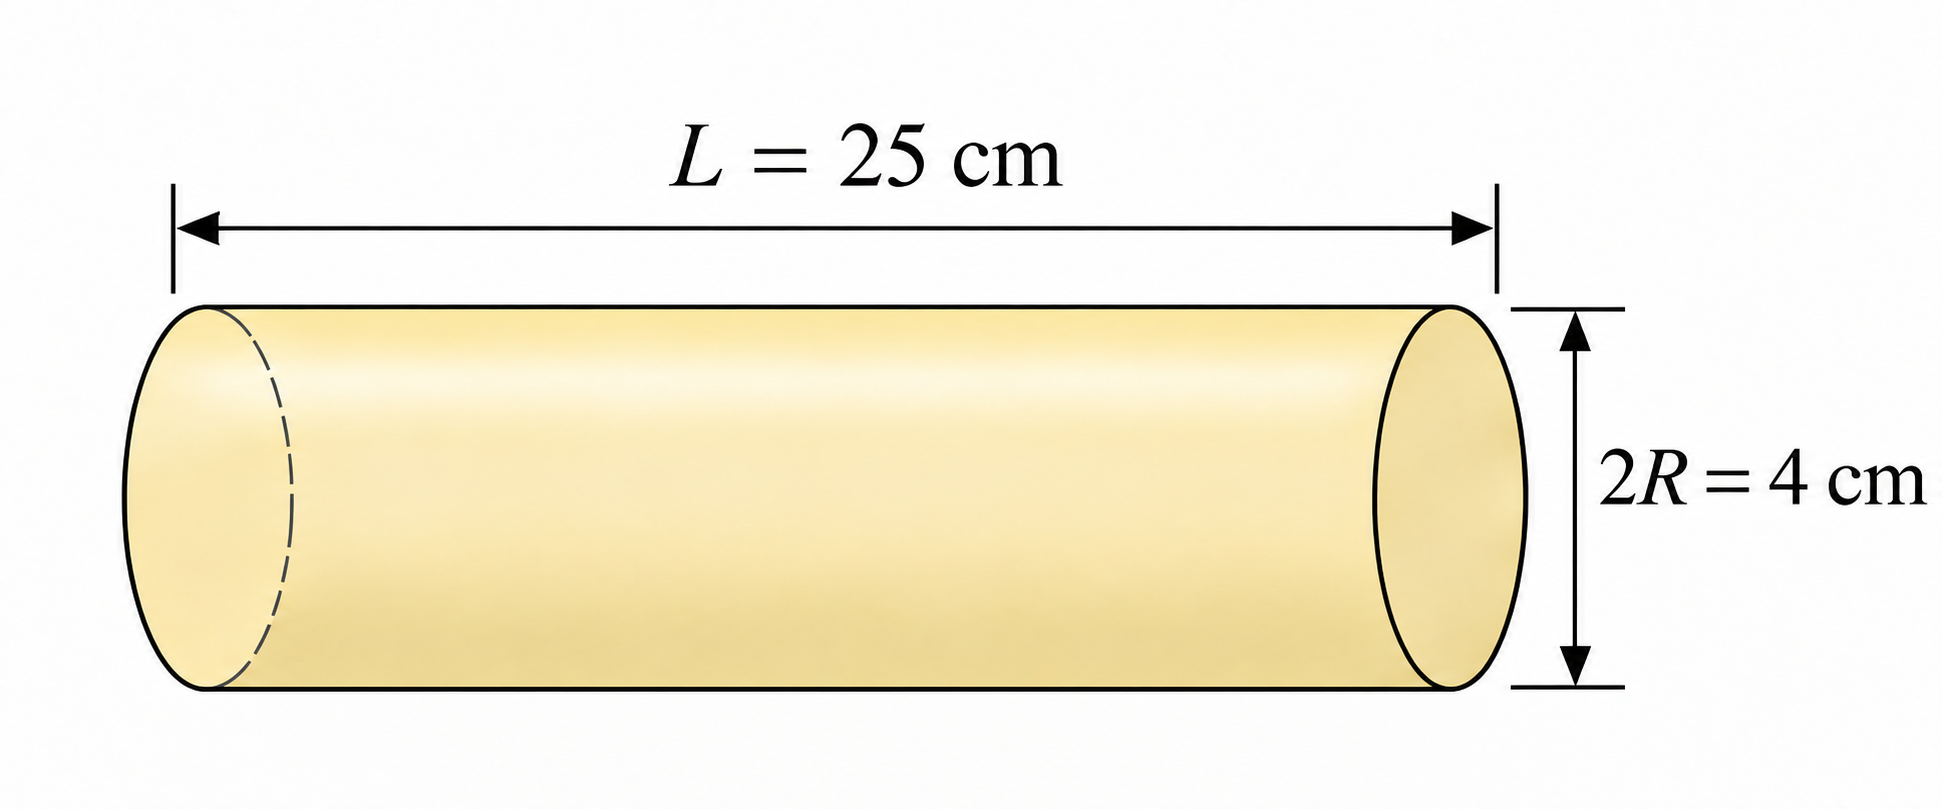
\includegraphics[width=0.8\textwidth]{figures/圆柱.png}
\caption{药材几何外形示意图}
\end{figure}

\textbf{问题一：}首先研究干燥开始后的$1800\,\mathrm{s}$预热阶段。利用附件1的烘房环境数据和附录2给出的物性参数，求解药材内部温度和含水率随时间及径向位置的分布。

\textbf{问题二：}在完整干燥过程的计算中，采用附录3的统一经验关系描述物性参数随状态的变化，建立温度场与含水率场的耦合模型。

\textbf{问题三：}在半径保持不变的条件下，以药材各处含水率均低于$0.15\,\mathrm{kg/kg}$作为干燥完成判据，确定达到该判据所需的时间。

\textbf{问题四：}进一步考虑药材失水后半径随时间收缩的情况，利用附件2的半径数据和附录4的经验关系修正传质计算域，重新确定达到$0.15\,\mathrm{kg/kg}$判据的干燥时长。

\section{问题分析}
\subsection{问题一}
问题一要求刻画预热平衡阶段药材内部温度和水分浓度随时间及径向位置的变化规律。由于药材可近似为均质、各向同性的细长圆柱体，其长度与半径之比为$12.5$，两个端面的总面积仅为侧面积的$8\%$，因此可忽略轴向梯度和端部效应，将问题简化为固定半径圆柱内的一维轴对称非稳态传热与传质问题(如图3)，从而将温度场与水分场作为两个相互并行的偏微分方程分别求解。对于温度场，根据Fourier导热定律和能量守恒建立圆柱坐标下的一维径向非稳态热传导方程，在圆柱中心设置对称边界，在药材表面设置Newton对流换热边界。对于水分场，根据Fick扩散定律和质量守恒建立径向扩散方程。为求解上述温度场和水分场的偏微分方程，本文采用径向有限体积法进行空间离散，并采用后向Euler全隐式格式进行时间离散与推进。

\begin{figure}[H]
\centering
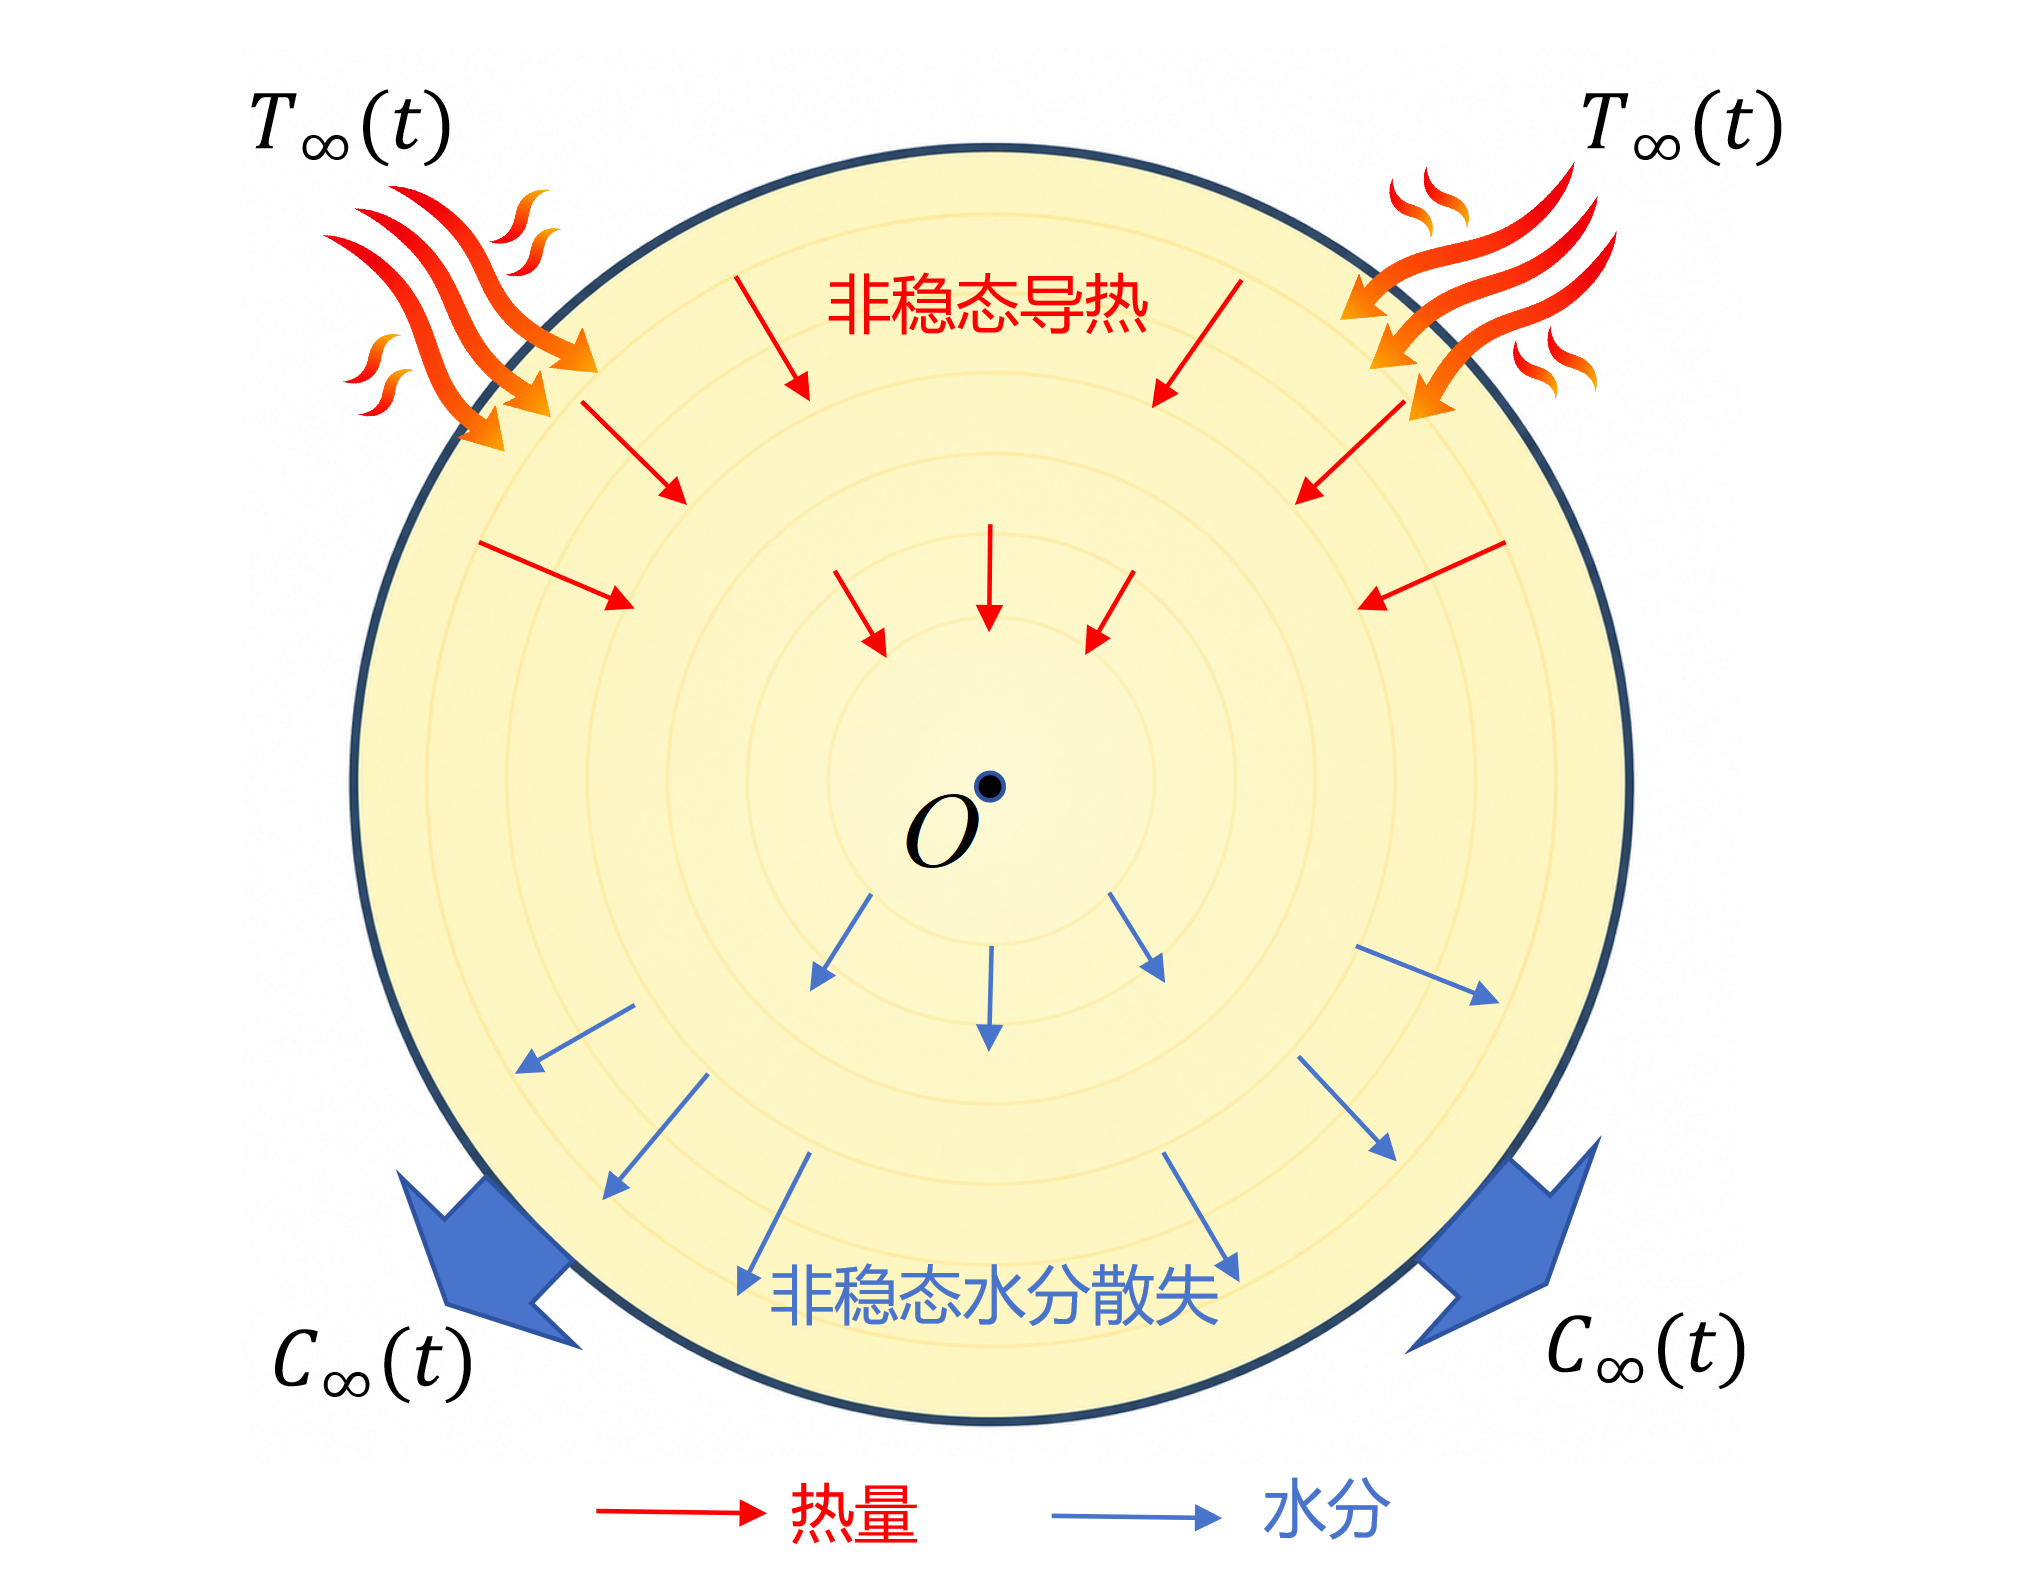
\includegraphics[width=0.8\textwidth]{figures/问题重述热量水分.png}
\caption{药材径向传热传质示意图}
\end{figure}


\subsection{问题二}
问题二沿用问题一建立的一维径向“传热-传质”模型，但进一步考虑药材物性参数随温度和含水率变化的影响。如图\ref{fig:q2-flowchart}所示，密度、比热容和导热系数由含水率决定，水分扩散系数则同时受含水率和绝对温度影响，因此温度场与水分场通过变物性参数形成间接双向耦合。模型从烘干初始状态开始计算，环境温度和水分浓度边界沿用分段线性插值结果。求解时采用与问题一一致的径向有限体积法和后向 Euler 全隐式格式，在每个时间层内交替更新变物性参数并采用 Picard 迭代求解，直至温度场和水分场同时收敛，进而获得前$3\,\mathrm{h}$内各时刻、各径向位置处的温度和水分浓度。

\begin{figure}[H]
\centering
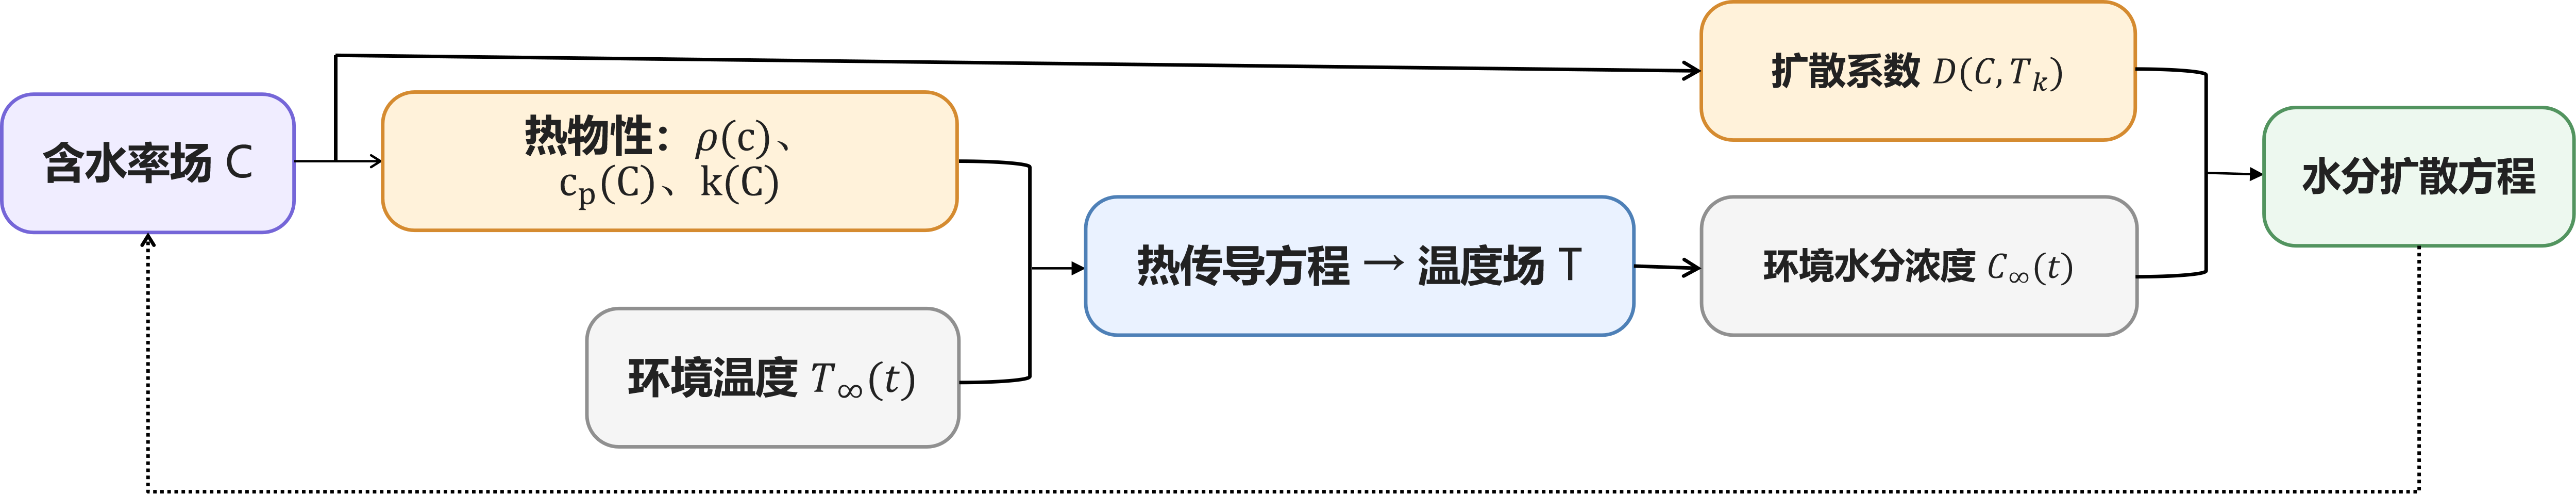
\includegraphics[width=0.95\textwidth]{figures/问题二流程图.png}
\caption{问题二热湿耦合计算流程图}
\label{fig:q2-flowchart}
\end{figure}

\subsection{问题三}
问题三中需要构建一个优化模型，求解螺距的最小值。首先，需明确优化模型的约束条件。根据问题一中在已知螺距下的计算结果及板凳的几何特性，可以缩小符合条件的螺距范围。通过计算龙头前把手到达调头空间边界的时刻，确定进入调头空间的最小螺距。在此过程中，还需利用问题二中的碰撞检测模型，确保在进入调头空间前未发生碰撞。模型求解采用变步长遍历的方法，逐步缩小步长以提高计算精度，结合启发式算法优化最短距离的计算过程。

\subsection{问题四}
问题四是在问题一模型基础上的扩展。基于题目提供的调头路径条件，通过几何相关知识可判断是否存在最优路径。由于路径较为复杂，可将其视作由四段曲线构成，并通过几何关系求解其中两段圆弧的参数方程。延续问题一的建模方式，先求出龙头前把手的每秒位置变化函数，再通过递推关系求解其余把手的位置函数。递推关系的求解需要区分相邻把手位于相同或不同曲线上的情况，速度的计算也需遵循类似的方法。

\subsection{问题五}
问题五的目的是建立一个优化模型，求解最大速度。首先需要在问题四的基础上，计算全过程中各把手的最大速度。其次需要对问题四的结果进行分析，结合物理规律，缩小搜索范围。最后依据速度最大值函数的特征，采用适当的算法求解最大速度。

\section{建模假设}
\begin{enumerate}[label=\arabic*.,leftmargin=2em,itemsep=0pt,topsep=0pt]
  \item \textbf{连续、均质、各向同性：}在宏观尺度上，将药材等效为连续、均质且各向同性的多孔介质，忽略纹理方向、孔隙结构及分层物性等信息以及各向异性的导热和扩散参数。
  \item \textbf{一维径向近似：}药材长度远大于半径，端面相对于侧面的面积较小，因此忽略周向变化和主体区域的轴向端部效应，只考虑径向传热与传质。
  \item \textbf{忽略蒸发散热：}水分蒸发会带走汽化潜热，但题目未给出汽化潜热、蒸发速率及相变动力学参数，因此温度方程中不显式加入蒸发吸热项；由此产生的影响作为模型误差处理。同时忽略体热源、化学反应热、辐射换热和热扩散引起的直接水分通量。
  \item \textbf{局部宏观平均：}将温度场 $T(r,t)$ 和干基含水率场 $C(r,t)$ 视为连续场变量，微观孔隙内的气液界面不单独解析，其影响等效包含在 $k$ 和 $D$ 中。

\end{enumerate}


\section{符号说明}
{\centering\textbf{表1\quad 符号说明}\par}
\begin{table}[H]
\centering
\renewcommand{\arraystretch}{1.12}
\begin{tabularx}{0.96\textwidth}{>{\centering\arraybackslash}p{0.18\textwidth}X>{\centering\arraybackslash}p{0.24\textwidth}}
\toprule
符号 & 含义 & SI单位 \\
\midrule
$L$ & 药材长度 & $\mathrm{m}$ \\
$R_0$ & 药材初始半径 & $\mathrm{m}$ \\
$r$ & 到圆柱中心轴的物理距离 & $\mathrm{m}$ \\
$R(t)$ & 当前药材半径；前三问为 $R_0$ & $\mathrm{m}$ \\
$t$ & 时间 & $\mathrm{s}$ \\
$T(r,t)$ & 药材温度 & $^\circ\mathrm{C}$ \\
$T_K(r,t)$ & 绝对温度，$T_K=T+273.15$ & $\mathrm{K}$ \\
$C(r,t)$ & 干基含水率，即水质量与绝干物质量之比 & $\mathrm{kg/kg}$ \\
$T_\infty(t)$ & 烘房环境温度 & $^\circ\mathrm{C}$ \\
$C_\infty(t)$ & 与表面传质模型匹配的环境等效含水率 & $\mathrm{kg/kg}$ \\
$\rho$ & 表观密度 & $\mathrm{kg/m^3}$ \\
$c_p$ & 比热容 & $\mathrm{J/(kg\cdot K)}$ \\
$k$ & 导热系数 & $\mathrm{W/(m\cdot K)}$ \\
$D$ & 有效水分扩散系数 & $\mathrm{m^2/s}$ \\
$h$ & 表面对流换热系数 & $\mathrm{W/(m^2\cdot K)}$ \\
$h_m$ & 表面对流传质系数 & $\mathrm{m/s}$ \\
$\xi$ & 第四问的无量纲材料坐标，$\xi=r/R(t)$ & $1$ \\
\bottomrule
\end{tabularx}
\end{table}

药材初始长度和半径分别为 $L=25\,\mathrm{cm}$、$R_0=2\,\mathrm{cm}$，初始状态为 $T(r,0)=28\,{}^\circ\mathrm{C}$、$C(r,0)=2.55\,\mathrm{kg/kg}$。
其中 $C$ 为干基含水率，数值 $2.55$ 表示每 $1\,\mathrm{kg}$ 绝干药材含 $2.55\,\mathrm{kg}$ 水。


\section{模型建立与求解}
\subsection{问题一模型的建立与求解}

\begin{figure}[H]
\centering
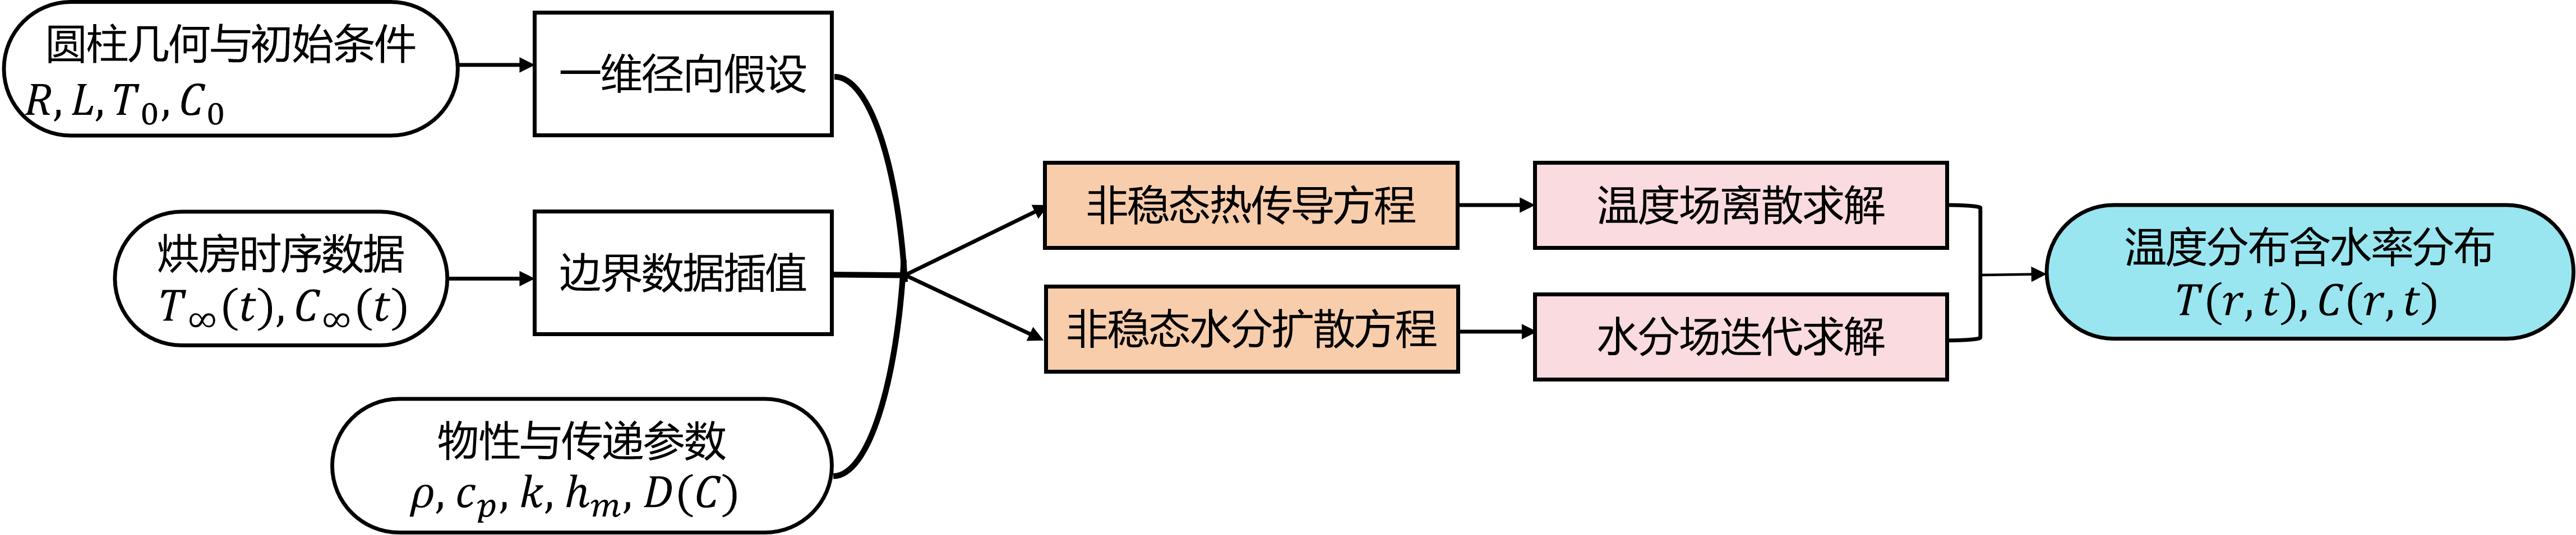
\includegraphics[width=0.9\textwidth]{figures/问题一流程图.png}
\caption{问题一流程图}
\end{figure}

\subsubsection{线性插值处理}
附件1给出的烘房温度和水分浓度为时间间隔$60\,\mathrm{s}$的离散采样序列，而数值离散的时间层间隔为$1\,\mathrm{s}$。为获得各计算时间层对应的边界状态，本文对该采样序列进行分段线性插值。设相邻采样时刻为$t_j$和$t_{j+1}$，则当$t\in[t_j,t_{j+1}]$时，有
\begin{equation}
\left\{
\begin{aligned}
T_\infty(t)&=T_{\infty,j}
+\frac{t-t_j}{t_{j+1}-t_j}
\left(T_{\infty,j+1}-T_{\infty,j}\right)\\
C_\infty(t)&=C_{\infty,j}
+\frac{t-t_j}{t_{j+1}-t_j}
\left(C_{\infty,j+1}-C_{\infty,j}\right)
\end{aligned}
\right.
\label{eq:environment-interpolation}
\end{equation}
该插值仅用于构造连续变化的边界条件，不改变附件1的原始采样数据。



\subsubsection{温度场模型}

为直观说明药材内部的传热、传质过程及其边界交换关系，本文通过图\ref{fig:q1-radial-process}展示一维径向非稳态热传导和水分扩散过程。图中药材中心采用轴对称条件，药材表面分别与烘房环境发生对流换热和对流传质，后文据此建立温度场和水分场控制方程。

\begin{figure}[H]
\centering
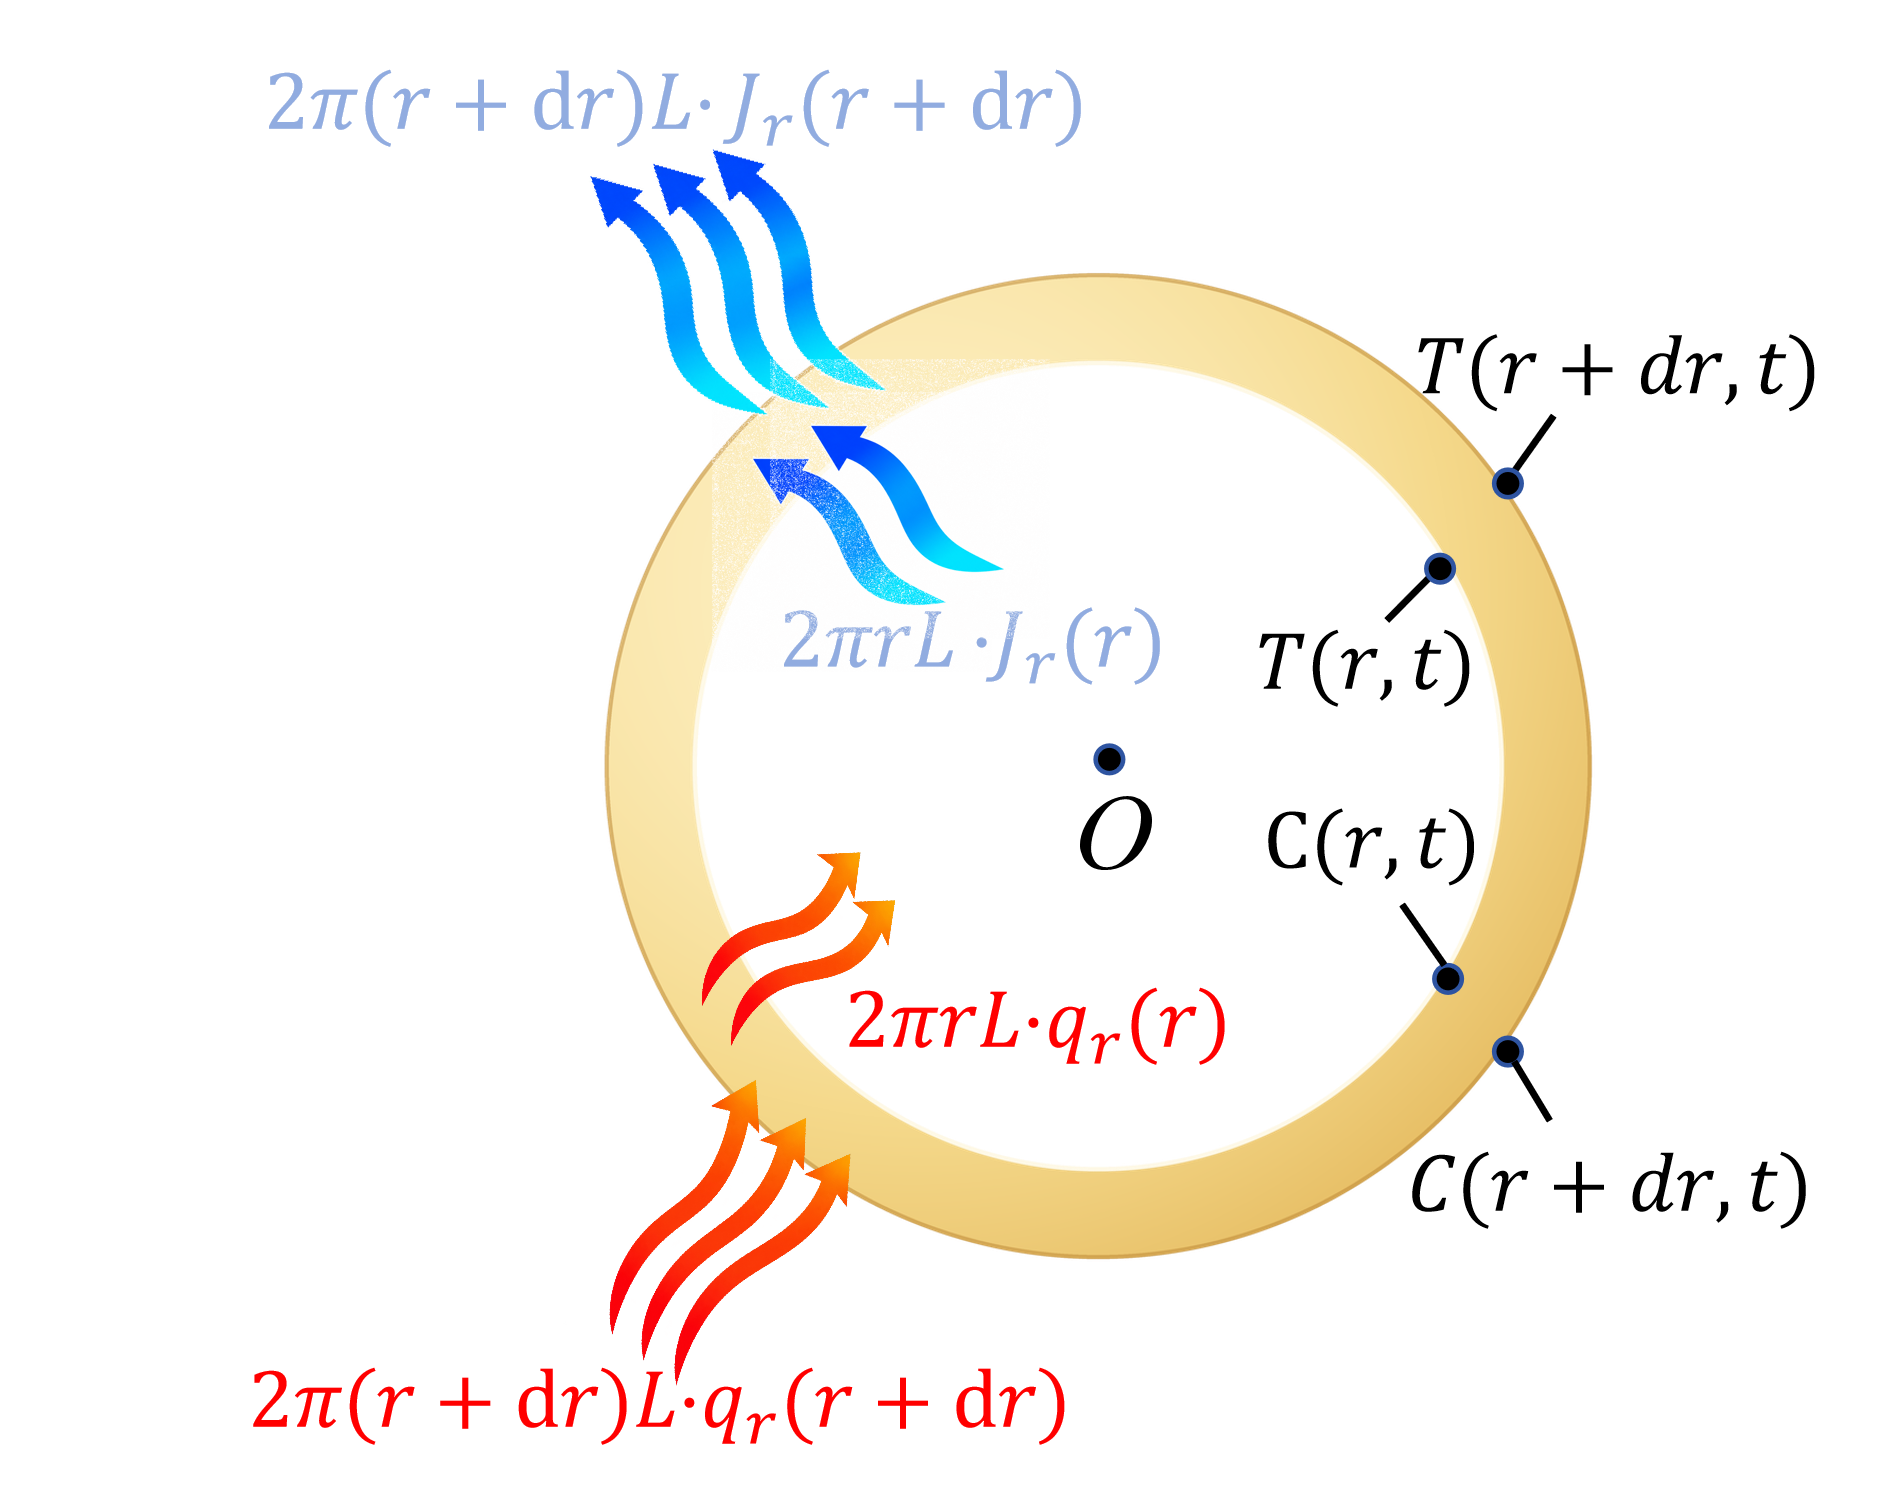
\includegraphics[width=0.8\textwidth]{figures/一维径向非稳态热传导示意图.png}
\caption{一维径向非稳态热传导和水分扩散示意图}
\label{fig:q1-radial-process}
\end{figure}

根据 Fourier 导热定律，药材内部的径向热流密度 $q_r$ 为 $-k\frac{\partial T}{\partial r}$。如图\ref{fig:q1-control-volume}所示，取半径为 $r$、厚度为 $\mathrm{d}r$、长度为 $L$ 的圆柱薄壳作为控制体，其体积 $\mathrm{d}V$为$2\pi rL\,\mathrm{d}r$。

\begin{figure}[H]
\centering
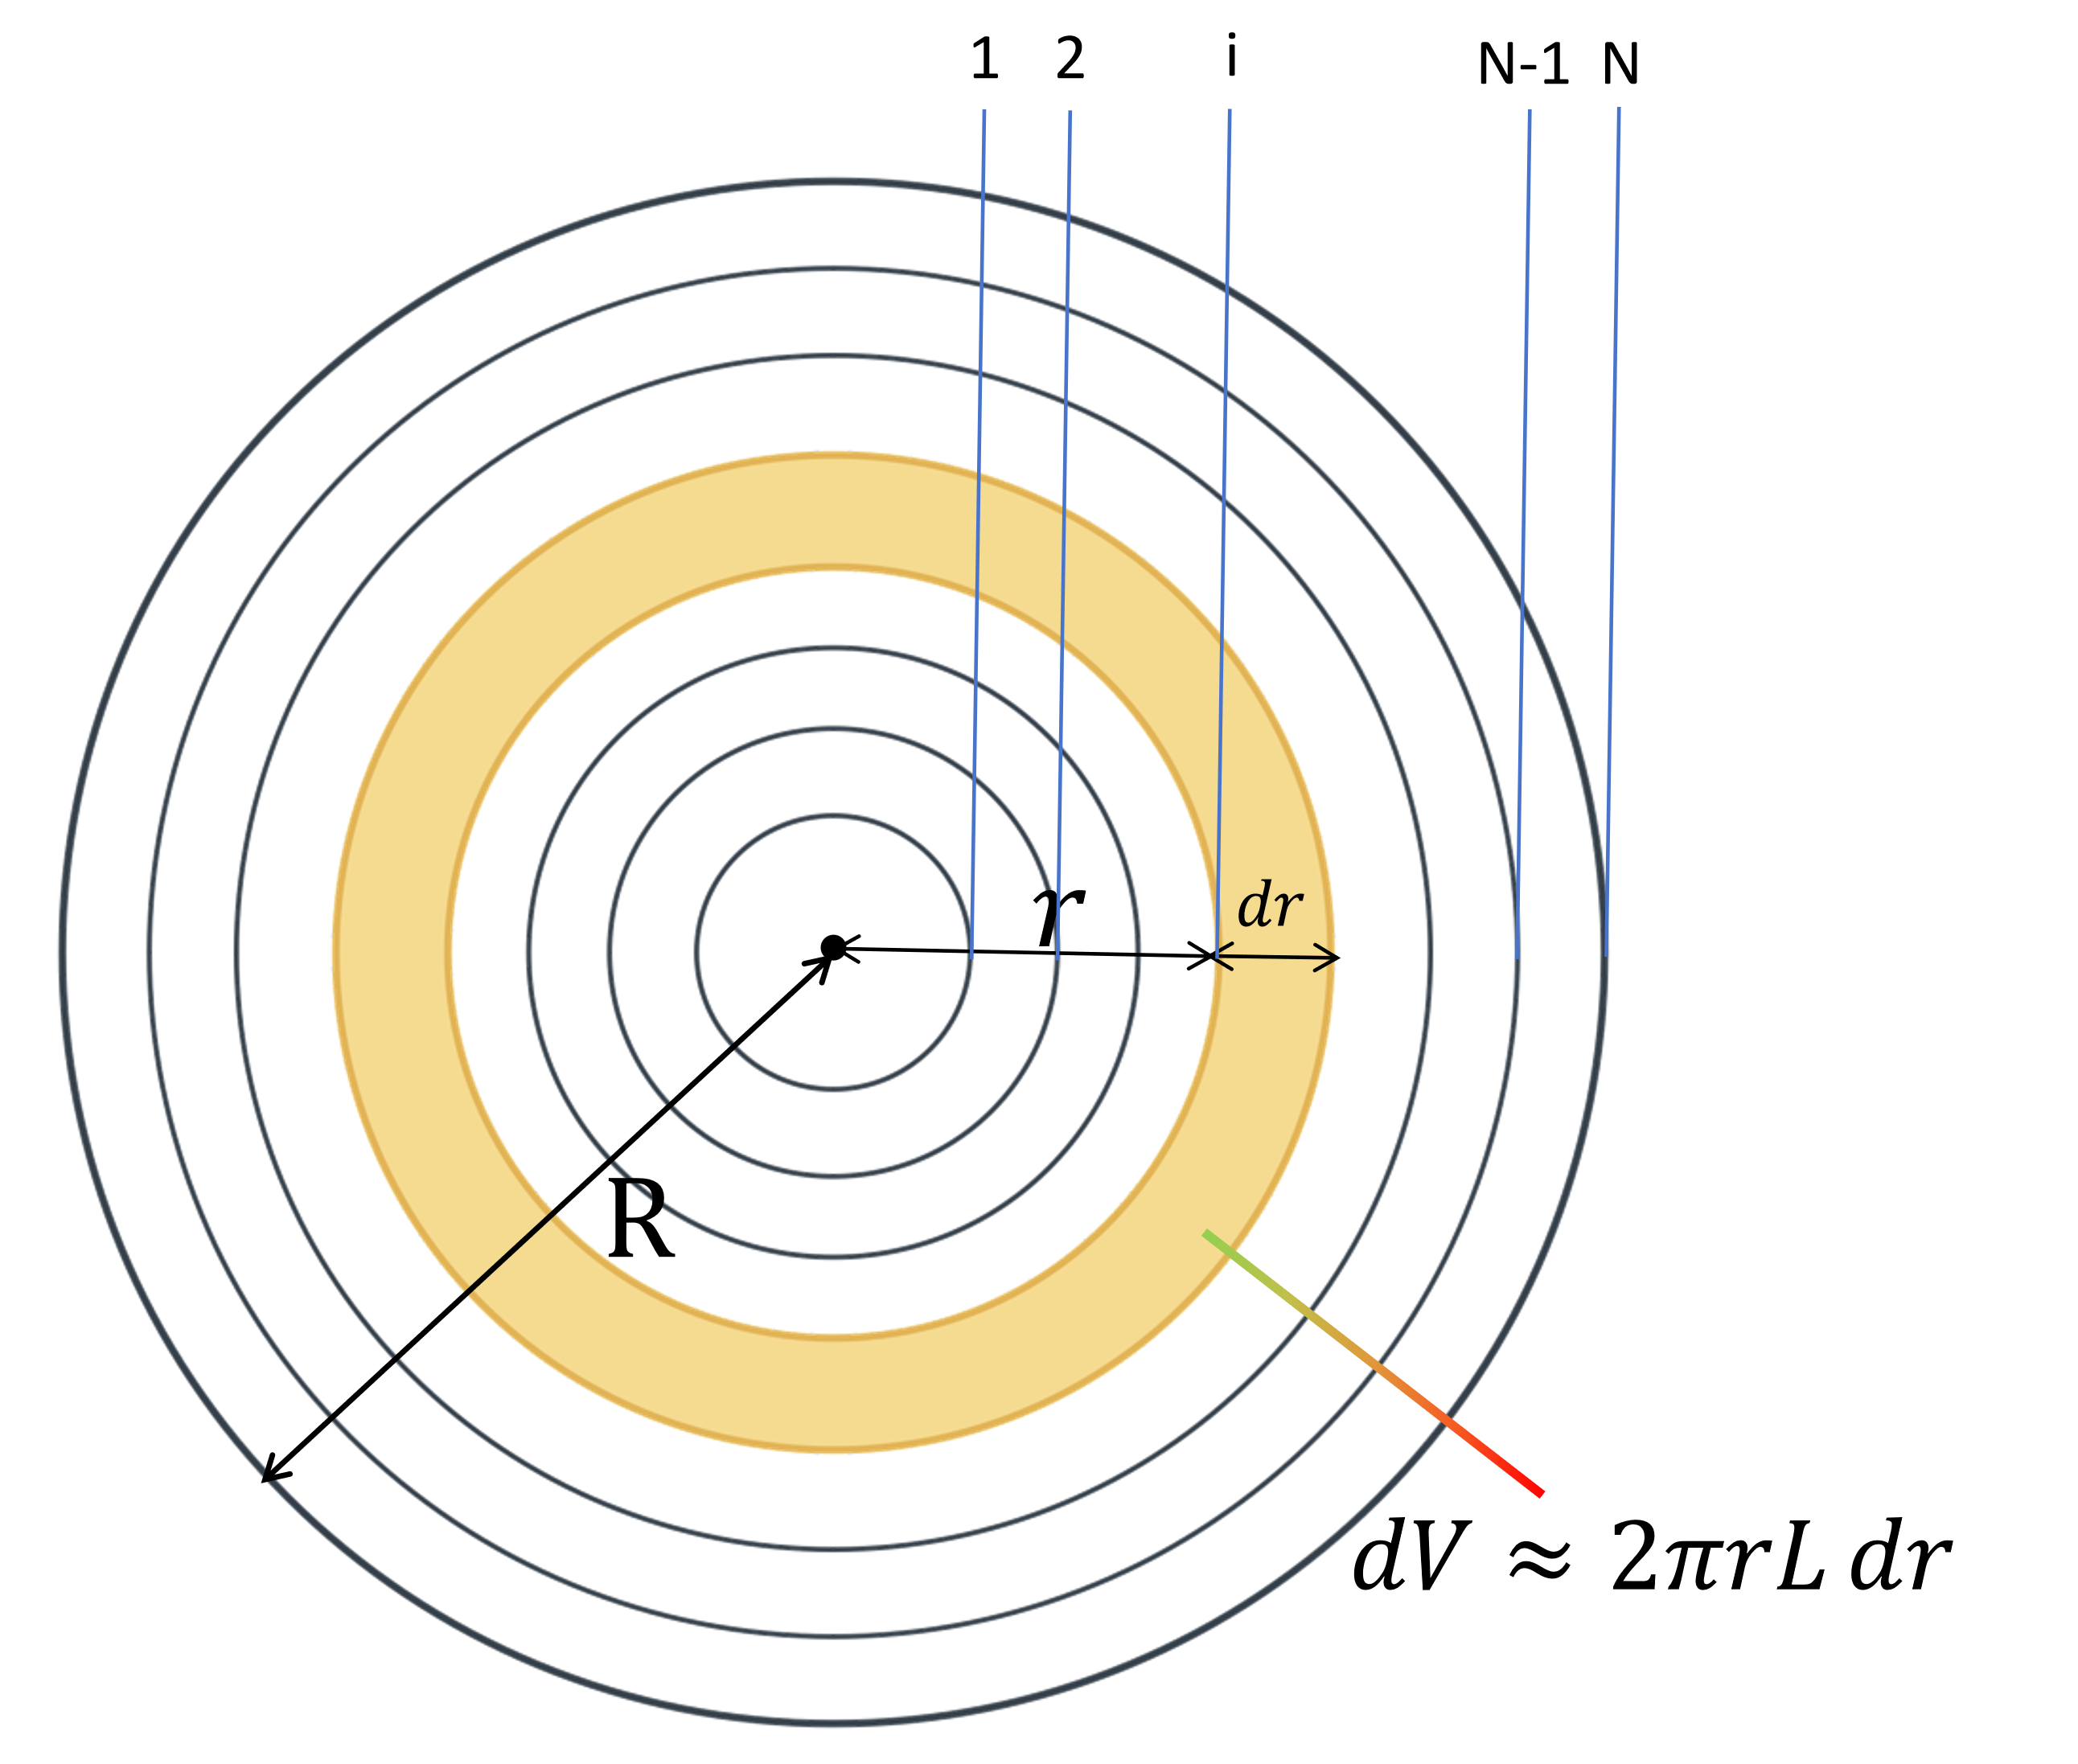
\includegraphics[width=0.8\textwidth]{figures/dV.png}
\caption{圆柱薄壳控制体示意图}
\label{fig:q1-control-volume}
\end{figure}

薄壳单位时间内的显热积累量为 $\rho c_p\,\mathrm{d}V\frac{\partial T}{\partial t}$。薄壳的净导热输入量等于内侧流入与外侧流出之差，由径向热流密度 $q_r$ 可写为 $-2\pi L\frac{\partial(rq_r)}{\partial r}\,\mathrm{d}r$。
根据能量守恒，显热积累量等于净导热输入量，约去公共因子 $2\pi L\,\mathrm{d}r$，得到圆柱坐标下的一维径向非稳态热传导方程：
\begin{equation}
\rho c_p\frac{\partial T}{\partial t}
=
\frac{1}{r}\frac{\partial}{\partial r}
\left(rk\frac{\partial T}{\partial r}\right)
\qquad 0<r<R,\quad 0<t\le1800\,\mathrm{s}.
\end{equation}
第一问中 $\rho$、$c_p$ 和 $k$ 均为常数，因此上式可写为：
\begin{equation}
\frac{\partial T}{\partial t}
=\alpha\left(
\frac{\partial^2T}{\partial r^2}
+\frac{1}{r}\frac{\partial T}{\partial r}
\right),
\qquad
\alpha=\frac{k}{\rho c_p}.
\end{equation}
代入题目给定的物性参数，得到热扩散率 $\alpha=1.6886\times10^{-7}\,\mathrm{m^2/s}$。

药材初始温度均匀，初始条件$T(r,0)=28\,{}^\circ\mathrm{C}$。
由于圆柱中心满足轴对称条件，有 $\left.\frac{\partial T}{\partial r}\right|_{r=0}=0$。
令 $T_s=T(R,t)$，药材表面向外的导热通量$q_{\mathrm{out}}$为 $-k\left.\frac{\partial T}{\partial r}\right|_{r=R}$。
根据 Newton 对流换热定律，环境向表面传出的热流为 $h(T_\infty-T_s)$。在药材与烘房气体的分界面上，根据能量守恒原理，药材内部导热通量与界面对流换热通量相等，得到表面对流换热边界条件：
\begin{equation}
-k\left.\frac{\partial T}{\partial r}\right|_{r=R}
=h\left[T_s-T_\infty(t)\right].
\end{equation}

\subsubsection{水分场模型}
根据 Fick 第一定律，药材内部的径向水分扩散通量 $J_r$ 为 $-D(C)\frac{\partial C}{\partial r}$。对同一圆柱薄壳控制体，含水率的积累量为 $2\pi rL\,\mathrm{d}r\frac{\partial C}{\partial t}$，水分的净扩散输入量为 $-2\pi L\frac{\partial(rJ_r)}{\partial r}\,\mathrm{d}r$。
根据质量守恒定律，约去公共因子并代入 Fick 定律，得到含水率的一维径向扩散方程
\begin{equation}
\frac{\partial C}{\partial t}
=
\frac{1}{r}\frac{\partial}{\partial r}
\left[rD(C)\frac{\partial C}{\partial r}\right]
\qquad 0<r<R,\quad 0<t\le1800\,\mathrm{s},
\end{equation}
其中水分扩散系数采用题目给定的经验公式：
\begin{equation}
D(C)=7\times10^{-9}
\exp\left(-\frac{0.89}{C}\right)\,\mathrm{m^2/s}.
\end{equation}

药材初始含水率均匀，因此 $C(r,0)=2.55$；圆柱中心满足无通量的轴对称条件 $\left.\frac{\partial C}{\partial r}\right|_{r=0}=0$。
初始时刻药材内部含水率为均匀分布，而表面与烘房环境的含水率通常不同，因此初始条件与对流边界在 $(R,0)$ 处可能不相容；这表示表面梯度将在 $t>0$ 的初始阶段迅速形成，并不构成模型错误。
令 $C_s=C(R,t)$。药材表面向外的扩散通量 $J_{\mathrm{out}}$ 为 $J_{\mathrm{out}}=-D(C_s)\left.\frac{\partial C}{\partial r}\right|_{r=R}$。
根据线性对流传质定律，表面向环境传出的水分通量为 $h_m(C_s-C_\infty)$，故表面传质边界为
\begin{equation}
-D(C_s)\left.\frac{\partial C}{\partial r}\right|_{r=R}
=h_m\left[C_s-C_\infty(t)\right].
\end{equation}

\subsubsection{数值离散与求解}

为满足题目对空间和时间输出分辨率的要求，本文直接采用题目规定的空间输出间隔构造径向计算网格。令空间步长为：
\begin{equation}
\Delta r=0.1\,\mathrm{cm}=1.0\times10^{-3}\,\mathrm{m},
\qquad
r_i=i\Delta r,\quad i=0,1,\ldots,20
\label{eq:q1-space-grid}
\end{equation}

时间步长取为：
\begin{equation}
\Delta t=1\,\mathrm{s},
\qquad
t_n=n\Delta t
\label{eq:q1-time-grid}
\end{equation}
其中，$n$为时间层编号。
采用$1\,\mathrm{s}$时间步长，一方面是为了满足题目每隔$1\,\mathrm{s}$输出完整结果的要求，另一方面能够使计算时间层准确承接附件1经分段线性插值后的边界条件。由于温度场和水分场均为扩散型方程，后向时间格式能够避免显式格式受到扩散稳定性条件的限制。

温度场和水分场均采用径向有限体积法离散，控制体取同心圆柱薄壳。为统一表示两个扩散方程，将其写为：
\begin{equation}
s\frac{\partial\phi}{\partial t}
=
\frac{1}{r}
\frac{\partial}{\partial r}
\left(
r\Gamma\frac{\partial\phi}{\partial r}
\right)
\label{eq:q1-unified-pde}
\end{equation}
其中，变量和参数对应关系为：
\begin{equation}
(\phi,s,\Gamma)=
\begin{cases}
(T,\rho c_p,k),&\text{温度场},\\
(C,1,D(C)),&\text{水分场}
\end{cases}
\label{eq:q1-unified-parameters}
\end{equation}

对内部控制体采用后向 Euler 全隐式格式，对式\eqref{eq:q1-unified-pde}进行有限体积离散，得到：
\begin{equation}
s_i
\frac{\phi_i^{n+1}-\phi_i^n}{\Delta t}
=
\frac{1}{r_i\Delta r}
\left[
r_{i+\frac12}\Gamma_{i+\frac12}^{n+1}
\frac{\phi_{i+1}^{n+1}-\phi_i^{n+1}}{\Delta r}
-
r_{i-\frac12}\Gamma_{i-\frac12}^{n+1}
\frac{\phi_i^{n+1}-\phi_{i-1}^{n+1}}{\Delta r}
\right]
\label{eq:q1-fvm-interior}
\end{equation}
其中，$i=1,2,\ldots,19$，$s_i$为节点$r_i$处的储存系数，$\Gamma_{i+\frac12}^{n+1}$为界面$r_{i+\frac12}$处的传递系数，且满足：
\begin{equation}
r_{i+\frac12}=r_i+\frac{\Delta r}{2}
\label{eq:q1-fvm-face}
\end{equation}
中心控制体不直接处理方程中的$1/r$项，而是利用圆柱中心的轴对称无通量条件得到中心节点离散式：
\begin{equation}
s_0
\frac{\phi_0^{n+1}-\phi_0^n}{\Delta t}
=
\frac{4\Gamma_{\frac12}^{n+1}}{\Delta r^2}
\left(\phi_1^{n+1}-\phi_0^{n+1}\right)
\label{eq:q1-fvm-center}
\end{equation}

记表面节点编号为$N=20$，并令$T_N^{n+1}=T(r_N,t_{n+1})$、$C_N^{n+1}=C(r_N,t_{n+1})$。表面控制体的外侧通量直接采用前文的Robin边界条件处理。对温度场，取由烘房指向药材内部为正的表面热通量，则有：
\begin{equation}
q_T^{n+1}
=
h\left[
T_\infty(t_{n+1})-T_N^{n+1}
\right]
\label{eq:q1-surface-heat-flux}
\end{equation}
对水分场，取由药材表面向环境为正的表面水分通量，则有：
\begin{equation}
q_C^{n+1}
=
h_m\left[
C_N^{n+1}-C_\infty(t_{n+1})
\right]
\label{eq:q1-surface-moisture-flux}
\end{equation}
将$q_T^{n+1}$和$q_C^{n+1}$分别作为表面控制体的外侧通量，按相应正方向代入表面离散方程，即可完成两类Robin边界条件的离散处理。

时间推进统一采用后向 Euler 全隐式格式，其中时间导数离散为$\frac{\phi_i^{n+1}-\phi_i^n}{\Delta t}$。
离散方程中的未知量均取$n+1$时刻。温度场中的$\rho$、$c_p$和$k$均为常数，因此每个时间层形成线性三对角方程组。水分场沿用前文给出的扩散系数关系，且该系数随含水率变化，因此在每个时间层内采用Picard迭代处理非线性：以第$m$次迭代的含水率场$C^{(m)}$计算扩散系数，在固定扩散系数下求解线性离散方程，得到新的含水率场$C^{(m+1)}$，再继续迭代，直至满足：
\begin{equation}
\max_i\left|C_i^{(m+1)}-C_i^{(m)}\right|<\varepsilon
\label{eq:q1-picard-convergence}
\end{equation}
其中，$m$为Picard迭代次数，$\varepsilon$为给定的收敛容差。界面扩散系数采用相邻节点扩散系数的调和平均，即：
\begin{equation}
D_{i+\frac12}
=
\frac{2D_iD_{i+1}}{D_i+D_{i+1}}
\label{eq:q1-harmonic-diffusivity}
\end{equation}
其中，$D_i$和$D_{i+1}$为当前迭代中相邻节点处的扩散系数。


\subsubsection{模型计算结果}

数值计算覆盖$t=0,1,\ldots,1800\,\mathrm{s}$的全部时间层和$r=0,0.1,\ldots,2.0\,\mathrm{cm}$的全部径向节点。从数值解中提取$t=100,300,600,900,1200,1500,1800\,\mathrm{s}$时，$r=0,0.5,1.0,1.5,2.0\,\mathrm{cm}$处的温度和水分浓度，结果分别列于表2和表3。

\begin{table}[H]
\centering
\renewcommand{\arraystretch}{1.25}
{\centering\textbf{表2\quad 30分钟内药材的温度}\par}
\vspace{0.4em}
\begin{tabularx}{0.9\textwidth}{|>{\centering\arraybackslash}p{0.20\textwidth}|>{\centering\arraybackslash}X|>{\centering\arraybackslash}X|>{\centering\arraybackslash}X|>{\centering\arraybackslash}X|>{\centering\arraybackslash}X|}
\hline
\multirow{2}{*}{时间/s} & \multicolumn{5}{c|}{到药材中心的距离/cm} \\
\cline{2-6}
& 0 & 0.5 & 1 & 1.5 & 2 \\
\hline
100  & 28.0001 & 28.0003 & 28.0040 & 28.0327 & 28.1801 \\
\hline
300  & 28.0408 & 28.0635 & 28.1514 & 28.3681 & 28.8489 \\
\hline
600  & 28.4533 & 28.5360 & 28.8039 & 29.3159 & 30.1652 \\
\hline
900  & 29.3243 & 29.4583 & 29.8755 & 30.6161 & 31.7304 \\
\hline
1200 & 30.5427 & 30.7098 & 31.2223 & 32.1126 & 33.4276 \\
\hline
1500 & 31.9957 & 32.1867 & 32.7660 & 33.7463 & 35.1203 \\
\hline
1800 & 33.5753 & 33.7720 & 34.3642 & 35.3621 & 36.7856 \\
\hline
\end{tabularx}
\end{table}

\begin{table}[H]
\centering
\renewcommand{\arraystretch}{1.25}
{\centering\textbf{表3\quad 30分钟内药材的水分浓度}\par}
\vspace{0.4em}
\begin{tabularx}{0.9\textwidth}{|>{\centering\arraybackslash}p{0.20\textwidth}|>{\centering\arraybackslash}X|>{\centering\arraybackslash}X|>{\centering\arraybackslash}X|>{\centering\arraybackslash}X|>{\centering\arraybackslash}X|}
\hline
\multirow{2}{*}{时间/s} & \multicolumn{5}{c|}{到药材中心的距离/cm} \\
\cline{2-6}
& 0 & 0.5 & 1 & 1.5 & 2 \\
\hline
100  & 2.5500 & 2.5500 & 2.5500 & 2.5500 & 2.2470 \\
\hline
300  & 2.5500 & 2.5500 & 2.5500 & 2.5492 & 2.0508 \\
\hline
600  & 2.5500 & 2.5500 & 2.5500 & 2.5353 & 1.8770 \\
\hline
900  & 2.5500 & 2.5500 & 2.5497 & 2.5045 & 1.7547 \\
\hline
1200 & 2.5500 & 2.5500 & 2.5482 & 2.4646 & 1.6586 \\
\hline
1500 & 2.5500 & 2.5499 & 2.5445 & 2.4206 & 1.5787 \\
\hline
1800 & 2.5500 & 2.5497 & 2.5383 & 2.3755 & 1.5102 \\
\hline
\end{tabularx}
\end{table}\

\noindent
同时，根据完整数值解绘制温度和水分浓度的三维时空分布曲面图，以及$t=0\,\mathrm{s}$、$900\,\mathrm{s}$和$1800\,\mathrm{s}$时的温度与水分浓度分布云图。三维曲面图见图\ref{fig:q1-3d-surfaces}，其中子图(a)为温度场，子图(b)为水分浓度场；分时刻云图见图\ref{fig:q1-clouds}，其中子图(a)为三个时刻的温度场，子图(b)为三个时刻的水分浓度场。

\begin{figure}[H]
\centering
\begin{subfigure}[b]{0.48\textwidth}
\centering
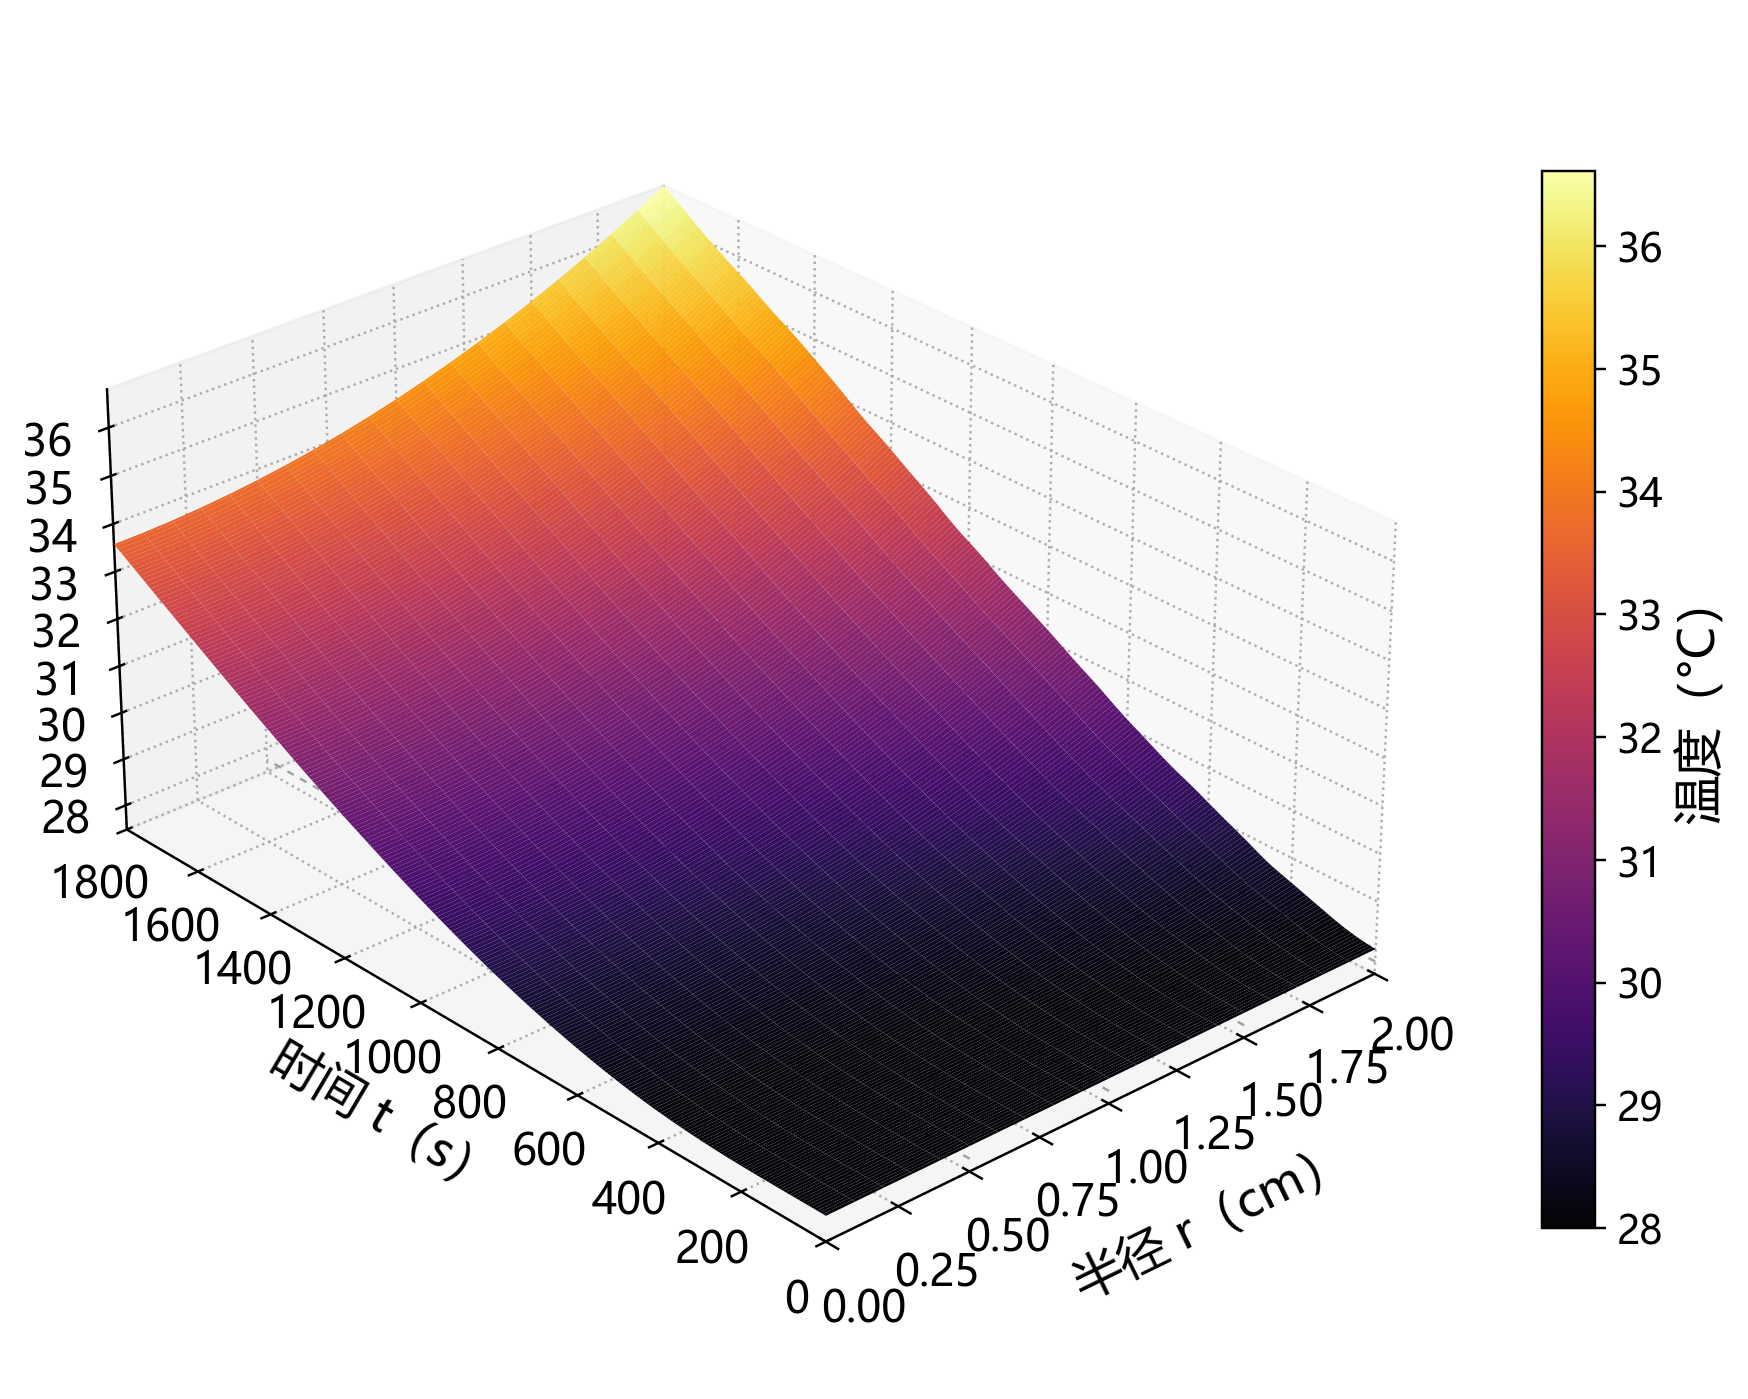
\includegraphics[width=\linewidth]{figures/温度三维时空分布曲面图.png}
\caption{温度三维时空分布曲面图}
\label{fig:q1-temperature-surface}
\end{subfigure}
\hfill
\begin{subfigure}[b]{0.48\textwidth}
\centering
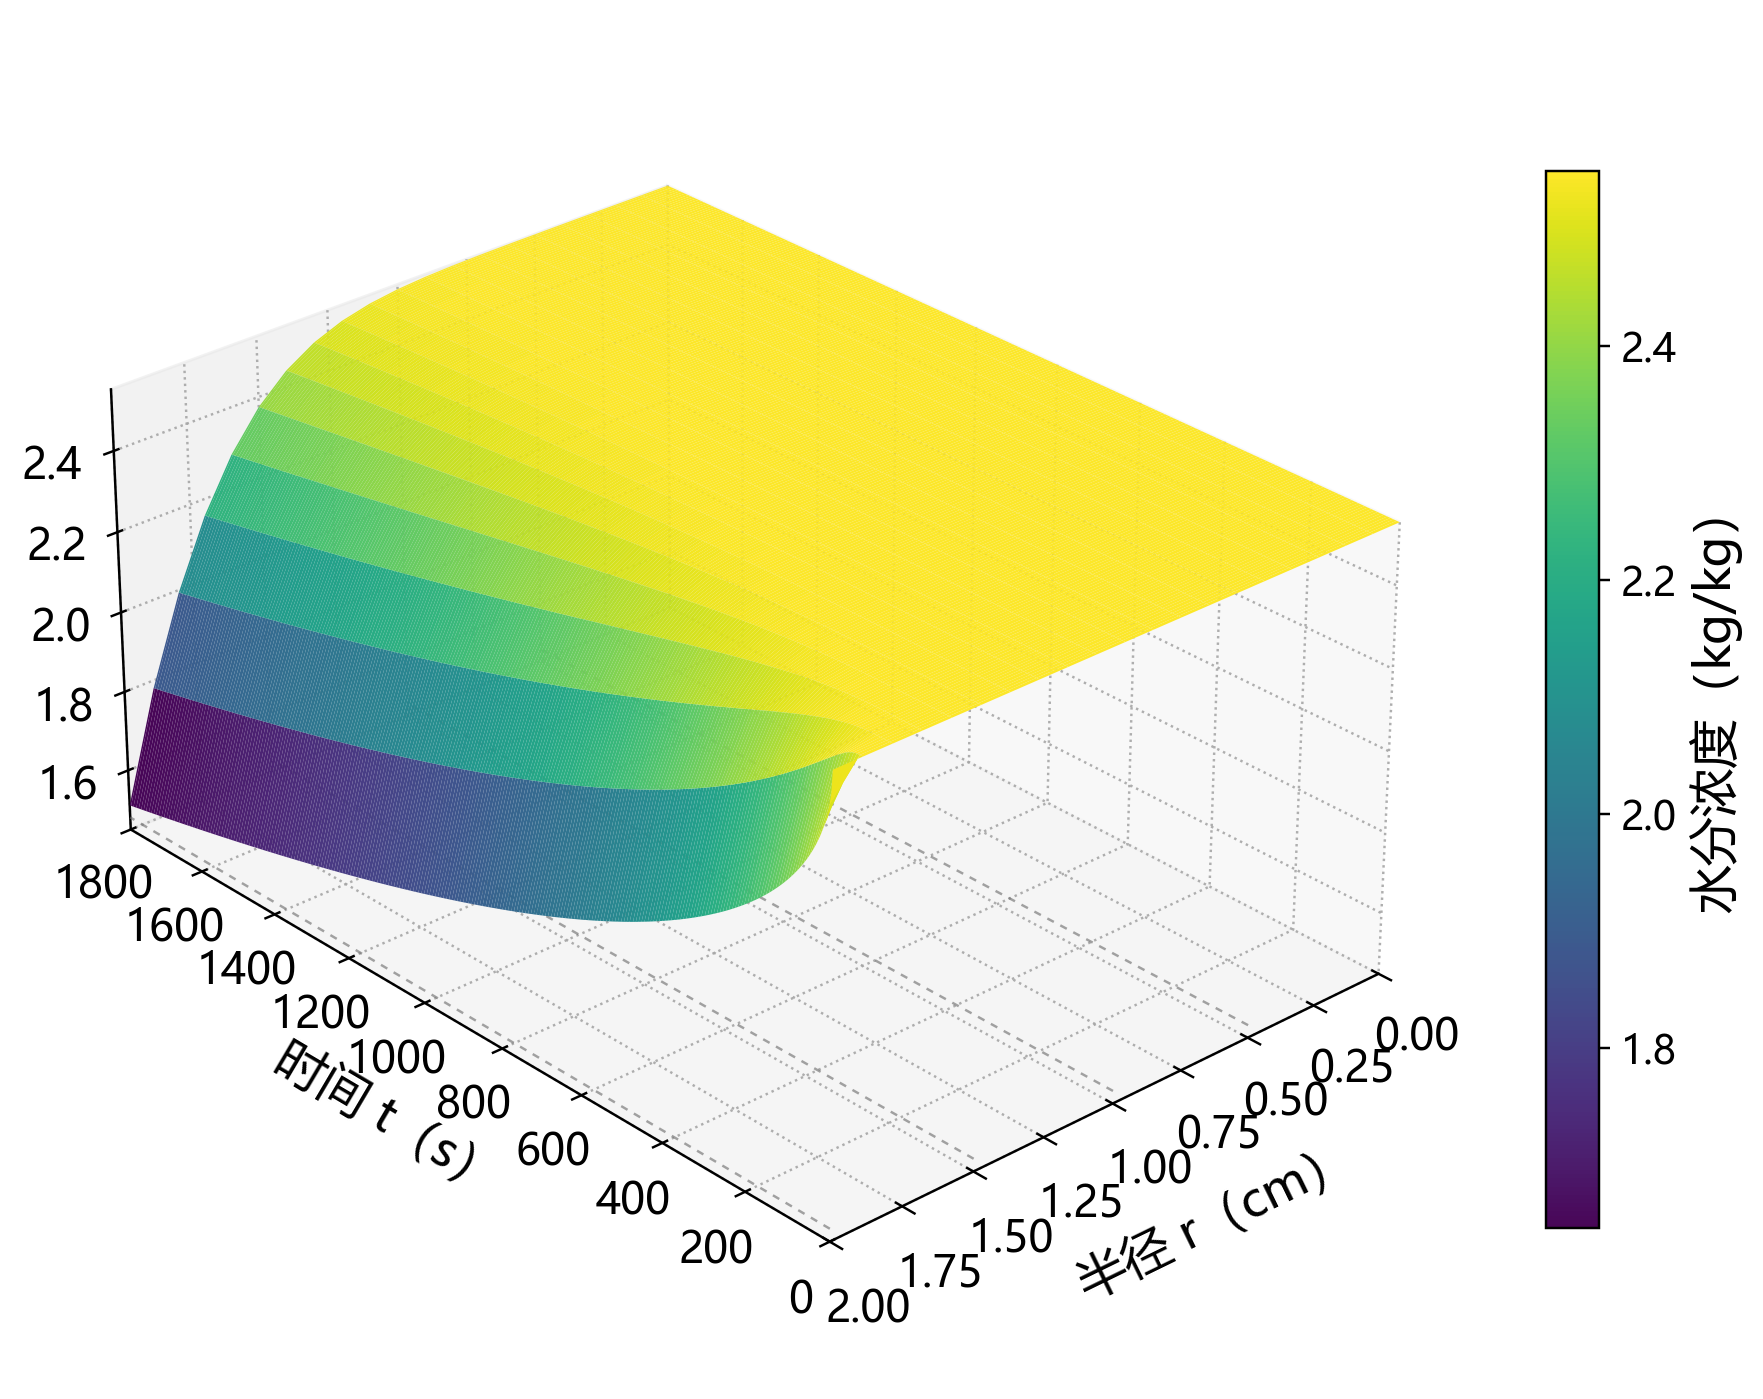
\includegraphics[width=\linewidth]{figures/水分浓度三维时空分布曲面图.png}
\caption{水分浓度三维时空分布曲面图}
\label{fig:q1-moisture-surface}
\end{subfigure}
\caption{温度和水分浓度三维时空分布曲面图}
\label{fig:q1-3d-surfaces}
\end{figure}

\begin{figure}[H]
\centering
\begin{subfigure}[b]{0.48\textwidth}
\centering
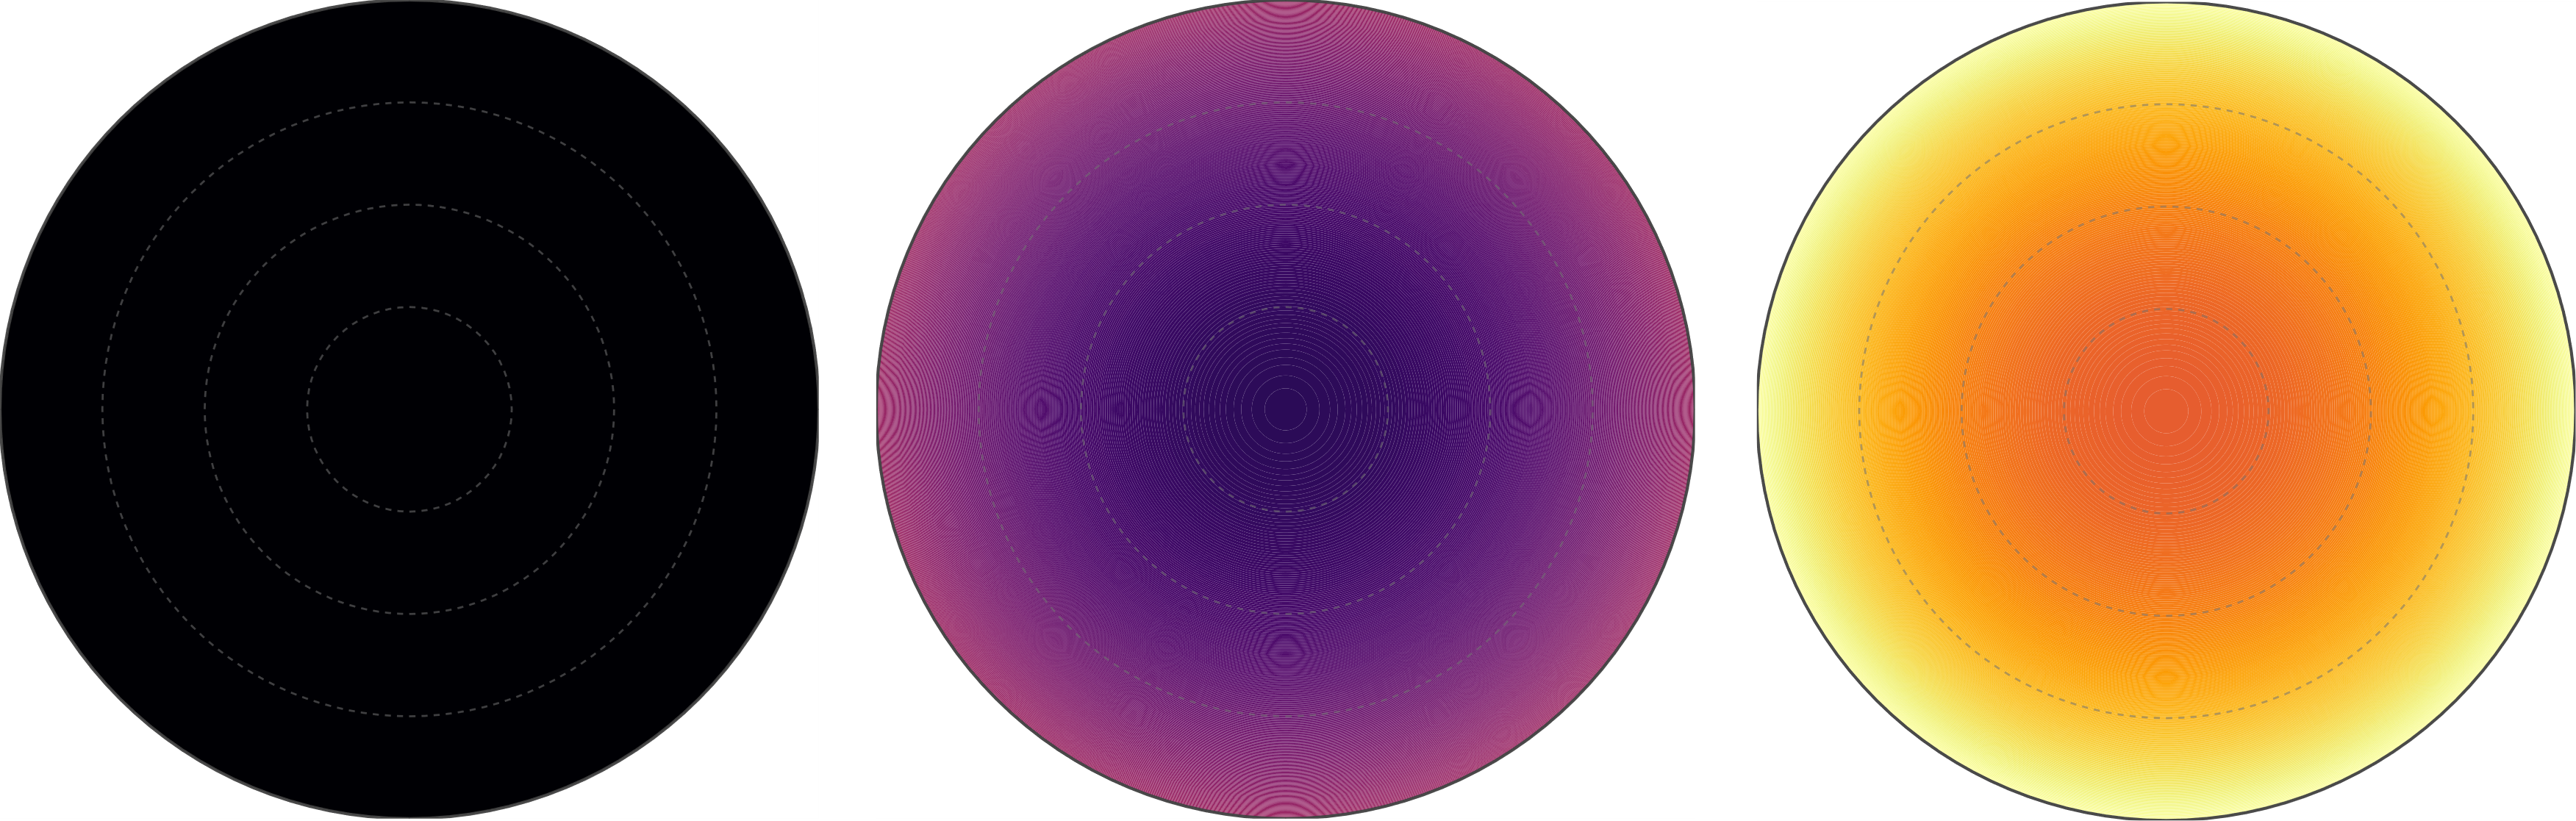
\includegraphics[width=\linewidth]{figures/云A.png}
\caption{$t=0\,\mathrm{s}$、$900\,\mathrm{s}$和$1800\,\mathrm{s}$时刻的温度分布云图}
\label{fig:q1-temperature-clouds}
\end{subfigure}
\hfill
\begin{subfigure}[b]{0.48\textwidth}
\centering
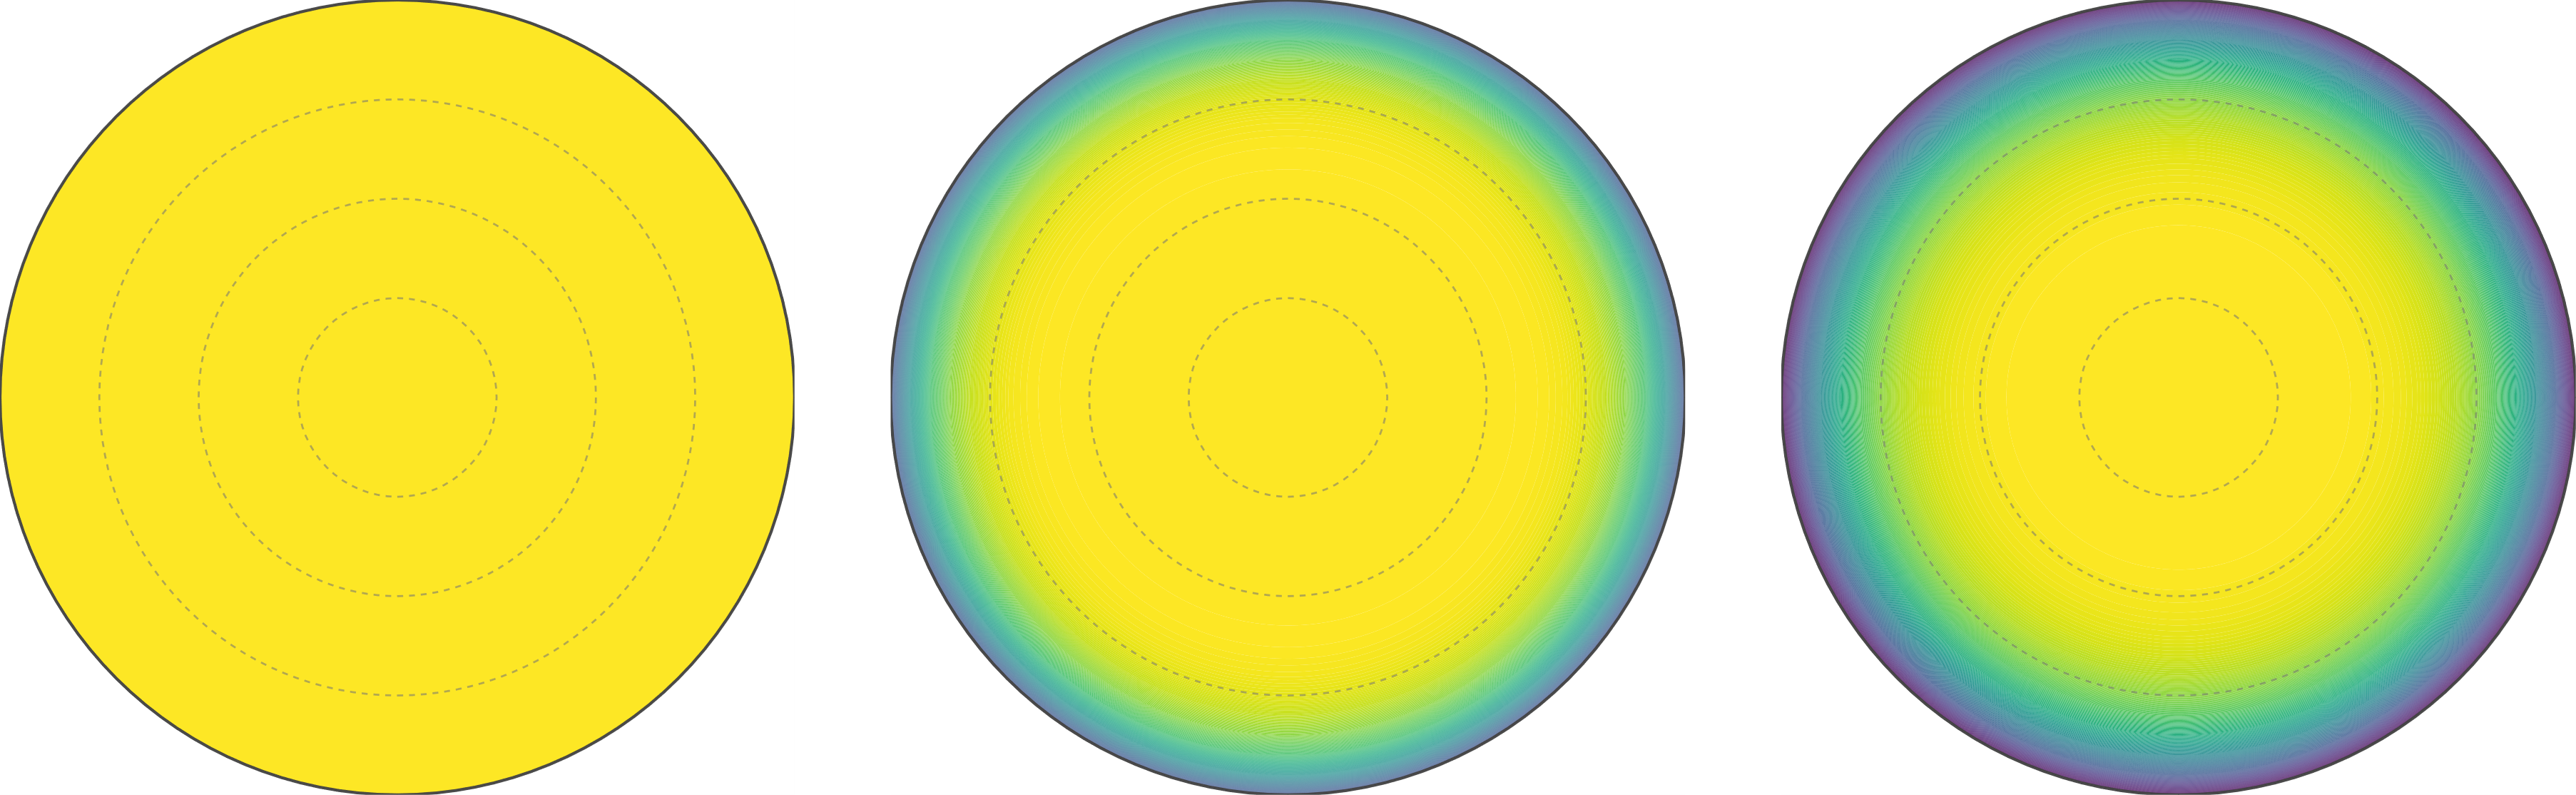
\includegraphics[width=\linewidth]{figures/云B.png}
\caption{$t=0\,\mathrm{s}$、$900\,\mathrm{s}$和$1800\,\mathrm{s}$时刻的水分浓度分布云图}
\label{fig:q1-moisture-clouds}
\end{subfigure}
\caption{不同时间的温度和水分浓度分布云图}
\label{fig:q1-clouds}
\end{figure}

\subsection{问题二模型的建立与求解}
\begin{figure}[H]
\centering
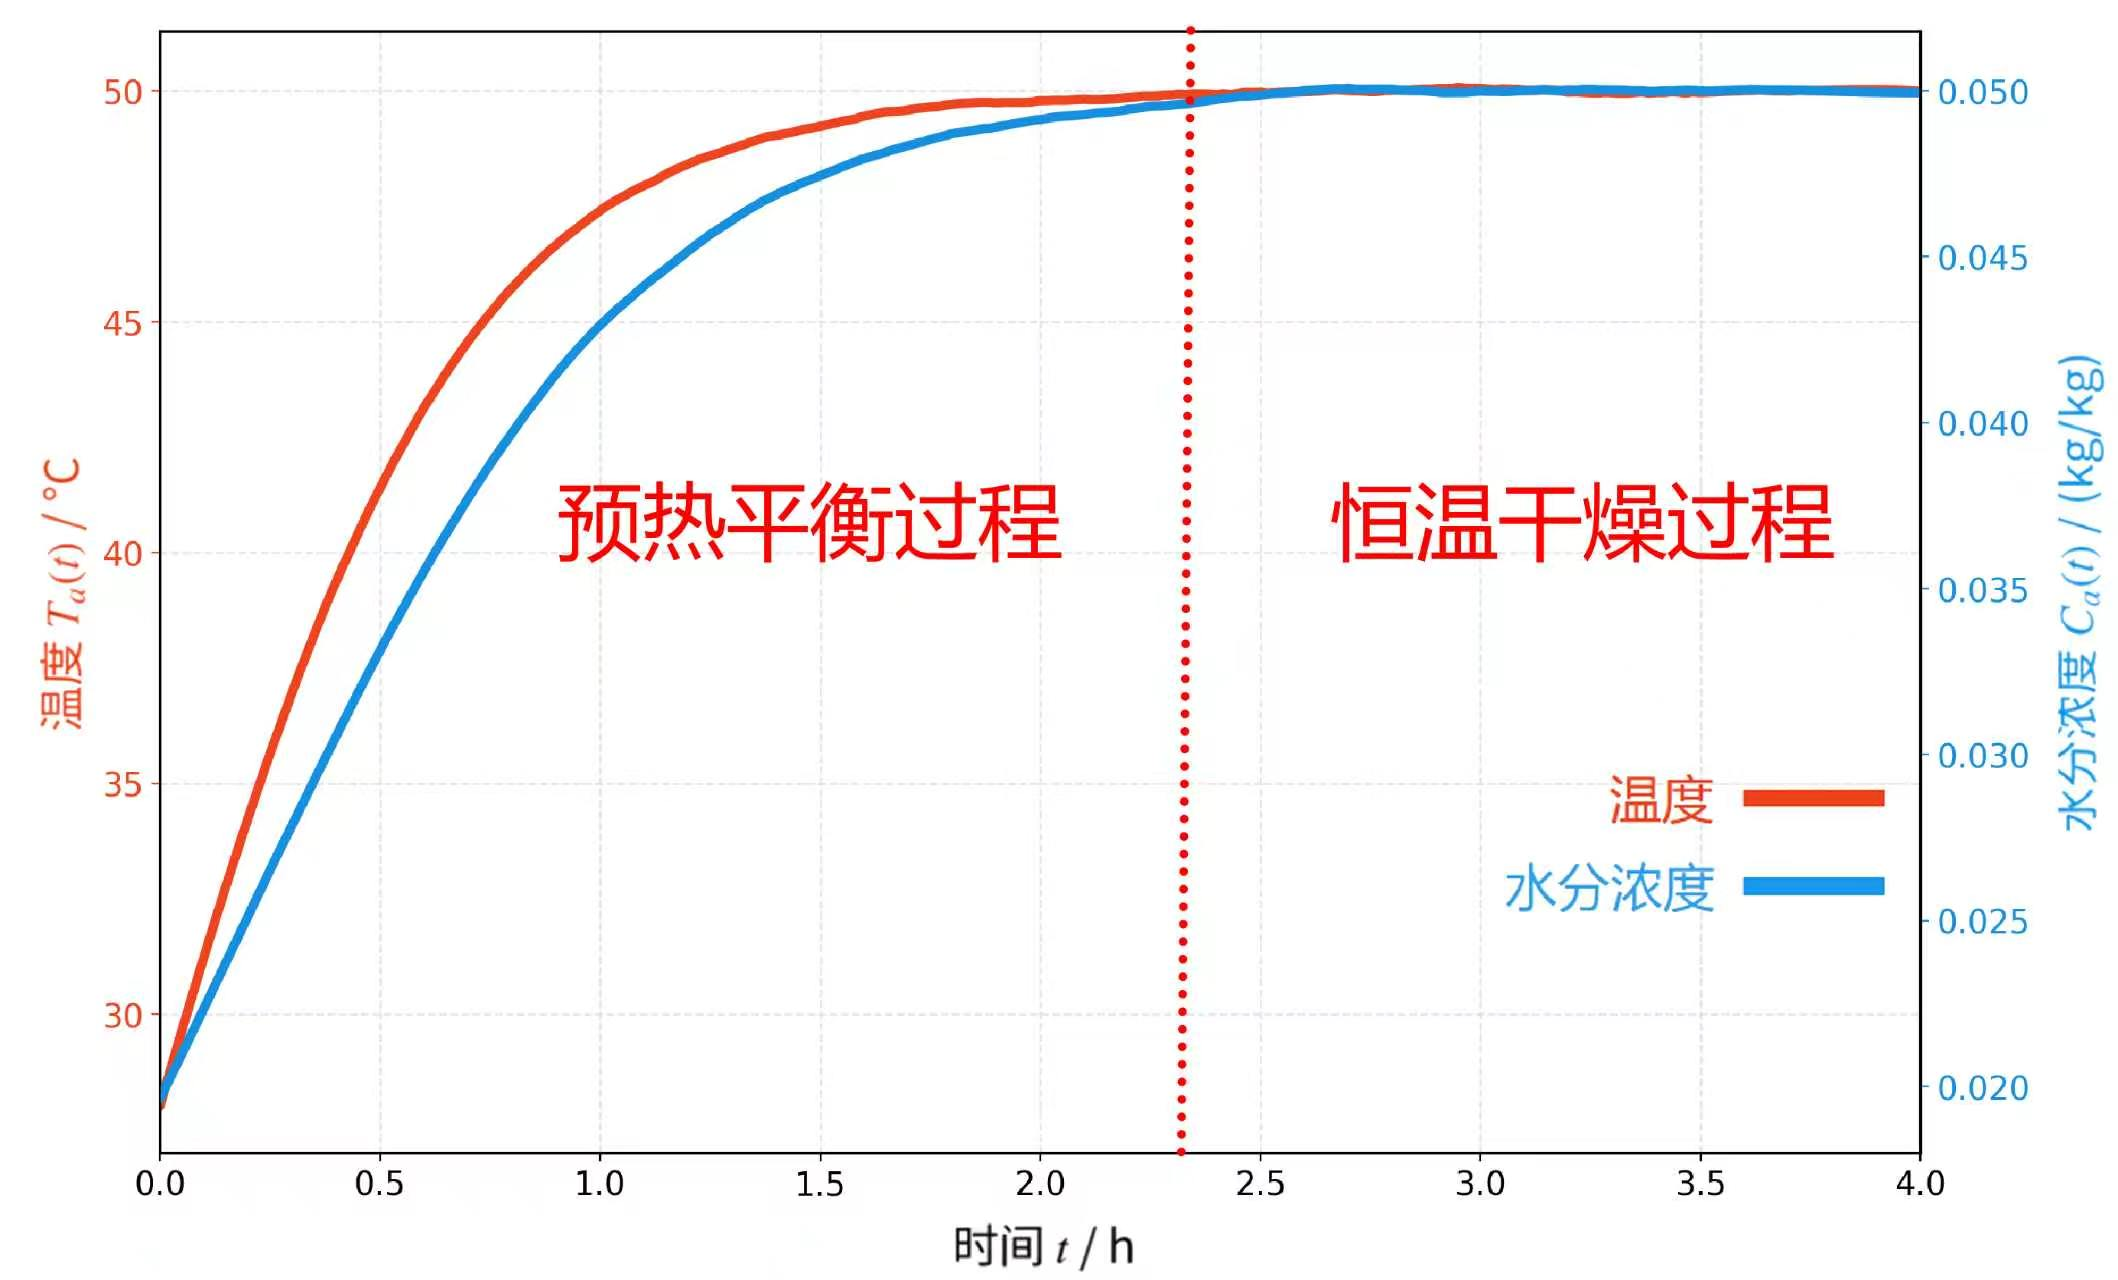
\includegraphics[width=0.8\textwidth]{figures/药材烘干过程示意图.png}
\caption{药材烘干过程示意图}
\end{figure}
\subsubsection{问题二模型的更新}

问题二沿用问题一建立的一维径向非稳态传热—传质模型，但进一步考虑药材物性参数随温度和含水率变化的影响。与问题一中物性参数固定的模型相比，问题二中的密度、比热容、导热系数和水分扩散系数均需采用题目给出的状态相关经验公式。因此，温度场与水分场通过变物性参数形成间接双向耦合。另外，问题二从烘干初始时刻重新计算，不将问题一在$1800\,\mathrm{s}$时的计算结果作为问题二的初始条件。

\subsubsection{变物性热湿耦合方程}

根据附录3，药材的变物性参数统一表示为
\begin{equation}
\left\{
\begin{aligned}
\rho(C)&=650+128C,\\
c_p(C)&=1450+2736\frac{C}{C+1},\\
k(C)&=0.21+0.38\frac{C}{C+1},\\
D(C,T_K)&=2.4\times10^{-3}
\exp\left(-\frac{0.45}{C}\right)
\exp\left(-\frac{3850}{T_K}\right)\,\mathrm{m^2/s}.
\end{aligned}
\right.
\label{eq:q2-variable-properties}
\end{equation}
其中，$\rho$、$c_p$和$k$分别表示表观密度、比热容和导热系数，$D$表示水分扩散系数，$T_K$为绝对温度。
扩散系数公式中的温度采用绝对温度，因此计算时使用：
\begin{equation}
T_K=T+273.15
\label{eq:q2-absolute-temperature}
\end{equation}

将上述变物性关系代入能量守恒方程和质量守恒方程，得到问题二的温度场控制方程：
\begin{equation}
\boxed{
\rho(C)c_p(C)\frac{\partial T}{\partial t}
=
\frac{1}{r}
\frac{\partial}{\partial r}
\left[
rk(C)\frac{\partial T}{\partial r}
\right]
}
\label{eq:q2-variable-heat}
\end{equation}
以及水分场控制方程：
\begin{equation}
\boxed{
\frac{\partial C}{\partial t}
=
\frac{1}{r}
\frac{\partial}{\partial r}
\left[
rD(C,T_K)\frac{\partial C}{\partial r}
\right]
}
\label{eq:q2-variable-moisture}
\end{equation}

含水率$C$决定$\rho(C)$、$c_p(C)$和$k(C)$，而温度$T$与含水率$C$共同决定扩散系数$D(C,T_K)$。因此，温度场和水分场需要在同一时间层内迭代求解。

\subsubsection{数值离散与耦合求解}

问题二沿用问题一的径向有限体积离散格式，空间步长取$\Delta r=0.1\,\mathrm{cm}$，时间步长取$\Delta t=1\,\mathrm{s}$。其中，$1\,\mathrm{s}$的时间步长既满足题目对完整结果的输出要求，又能够与分段线性插值后的环境边界条件逐时间层对应；同时采用后向 Euler 格式以提高扩散型方程在变物性条件下的数值稳定性。计算节点为：
\begin{equation}
\Delta r=0.1\,\mathrm{cm}=1.0\times10^{-3}\,\mathrm{m},
\qquad
r_i=i\Delta r,\quad i=0,1,\ldots,20
\label{eq:q2-space-grid}
\end{equation}
时间步长为：
\begin{equation}
\Delta t=1\,\mathrm{s}
\label{eq:q2-time-grid}
\end{equation}

为统一表示问题二中的温度场和水分场，问题一中的统一离散形式仍然适用，仅将储存系数和传递系数替换为：
\begin{equation}
(s,\Gamma)=
\begin{cases}
(\rho(C)c_p(C),k(C)),&\text{温度场},\\
(1,D(C,T_K)),&\text{水分场}
\end{cases}
\label{eq:q2-variable-parameters}
\end{equation}
内部控制体、中心控制体和表面控制体的有限体积离散分别沿用式\eqref{eq:q1-fvm-interior}、式\eqref{eq:q1-fvm-center}以及问题一中的表面Robin边界处理。由于离散方程中的物性参数依赖于当前温度场和含水率场，每个时间层内采用Picard迭代处理非线性耦合。首先根据当前含水率更新$\rho$、$c_p$和$k$，求解温度场；随后将更新后的温度转换为绝对温度，并结合含水率计算扩散系数$D$，再求解水分场。当相邻两次迭代的温度场和含水率场最大增量均小于给定容差时，认为当前时间层收敛，即：
内部控制体、中心控制体和表面控制体的有限体积离散分别沿用式\eqref{eq:q1-fvm-interior}、式\eqref{eq:q1-fvm-center}以及问题一中的表面Robin边界处理。后向 Euler 离散中，场变量及其对应的变物性参数均取当前时间层$n+1$的值。由于离散方程中的物性参数依赖于当前温度场和含水率场，每个时间层内采用Picard迭代处理非线性耦合。首先根据当前含水率更新$\rho$、$c_p$和$k$，求解温度场；随后将更新后的温度转换为绝对温度，并结合含水率计算扩散系数$D$，再求解水分场。当相邻两次迭代的温度场和含水率场最大增量均小于给定容差时，认为当前时间层收敛，即：
\begin{equation}
\max_i\left|T_i^{(m+1)}-T_i^{(m)}\right|<\varepsilon_T,
\qquad
\max_i\left|C_i^{(m+1)}-C_i^{(m)}\right|<\varepsilon_C
\label{eq:q2-picard}
\end{equation}
其中，$m$为时间层内的Picard迭代次数，$\varepsilon_T$和$\varepsilon_C$分别为温度场与含水率场的收敛容差。水分场界面扩散系数仍采用相邻节点扩散系数的调和平均：
\begin{equation}
D_{i+\frac12}
=
\frac{2D_iD_{i+1}}{D_i+D_{i+1}}
\label{eq:q2-harmonic-diffusivity}
\end{equation}

\subsubsection{模型计算结果}

问题二的数值计算覆盖全部时间层$t=0,1,\ldots,10800\,\mathrm{s}$和全部径向节点$r=0,0.1,\ldots,2.0\,\mathrm{cm}$。基于全部时间层和全部径向节点的数值计算结果，绘制温度场和水分浓度场在各径向位置上的时间变化折线图，如图\ref{fig:q2-results}所示，其中子图(a)为温度场，子图(b)为水分浓度场；同时提取$0.5,1.0,1.5,2.0,2.5,3.0\,\mathrm{h}$时，$r=0,0.5,1.0,1.5,2.0\,\mathrm{cm}$处的温度和水分浓度，结果分别列于表\ref{tab:q2-temperature}和表\ref{tab:q2-moisture}。

\begin{figure}[H]
\centering
\begin{subfigure}[b]{0.48\textwidth}
\centering
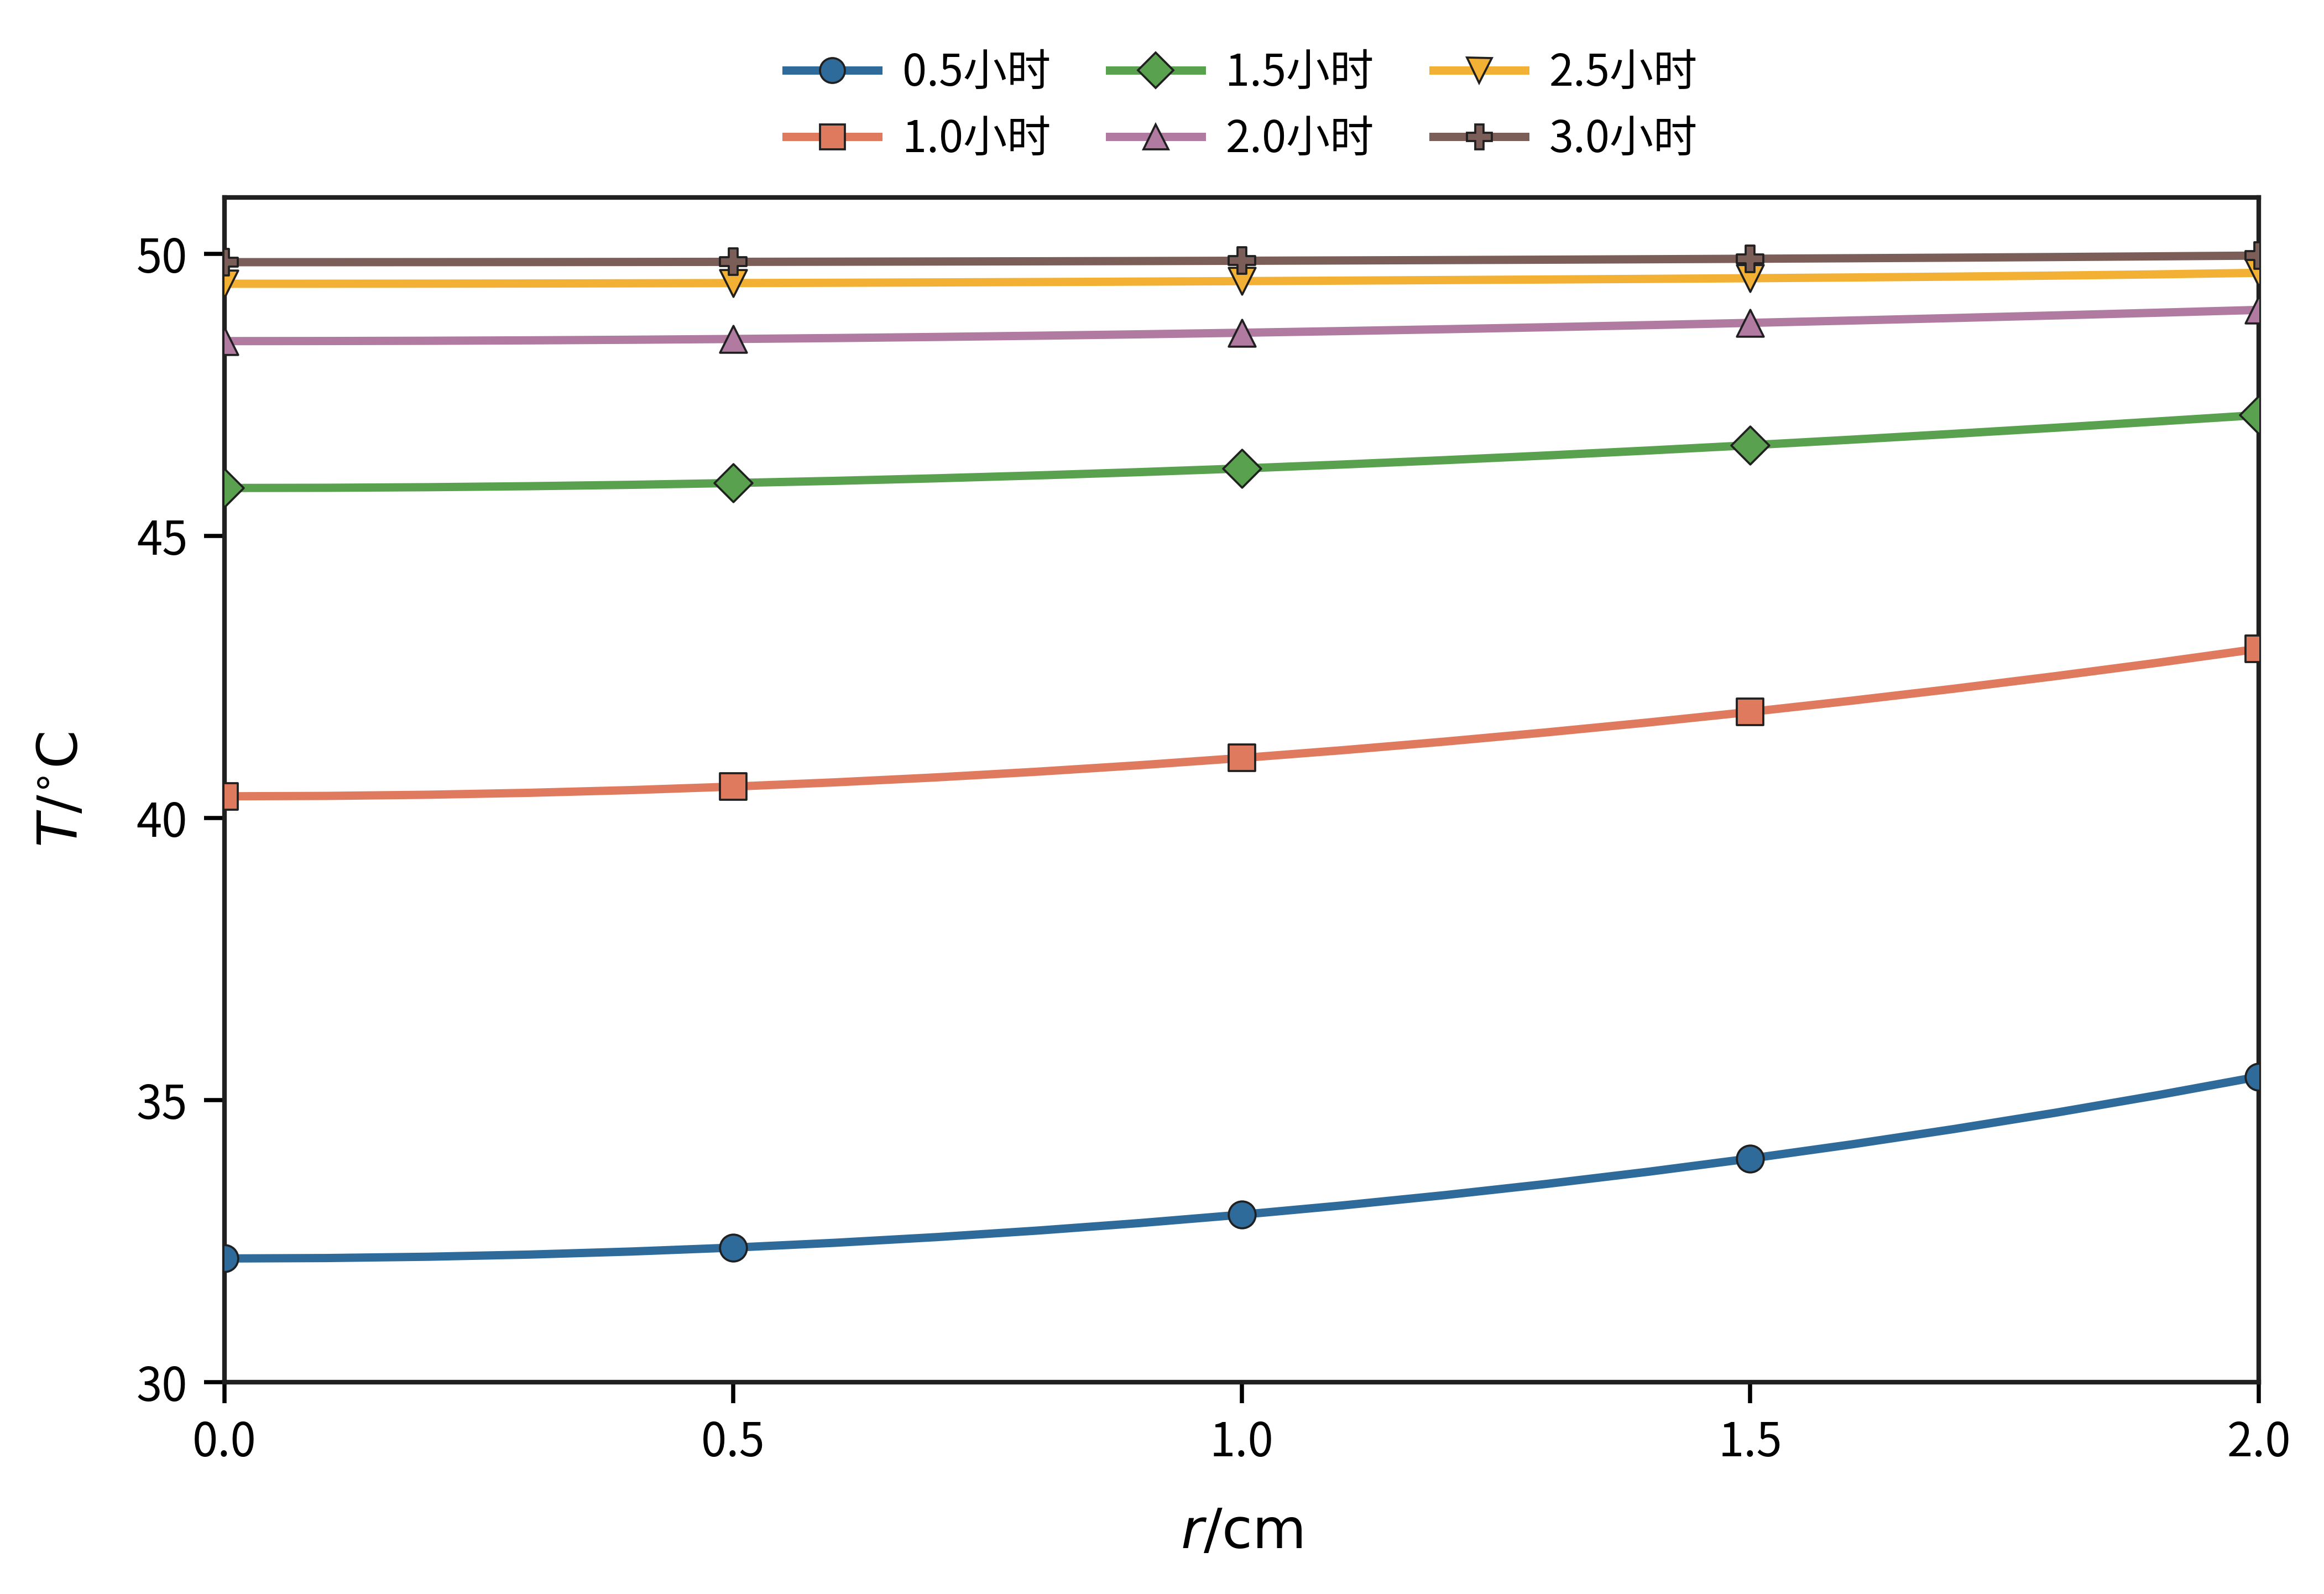
\includegraphics[width=\linewidth]{figures/问题二温度.png}
\caption{温度变化折线图}
\label{fig:q2-temperature-curves}
\end{subfigure}
\hfill
\begin{subfigure}[b]{0.48\textwidth}
\centering
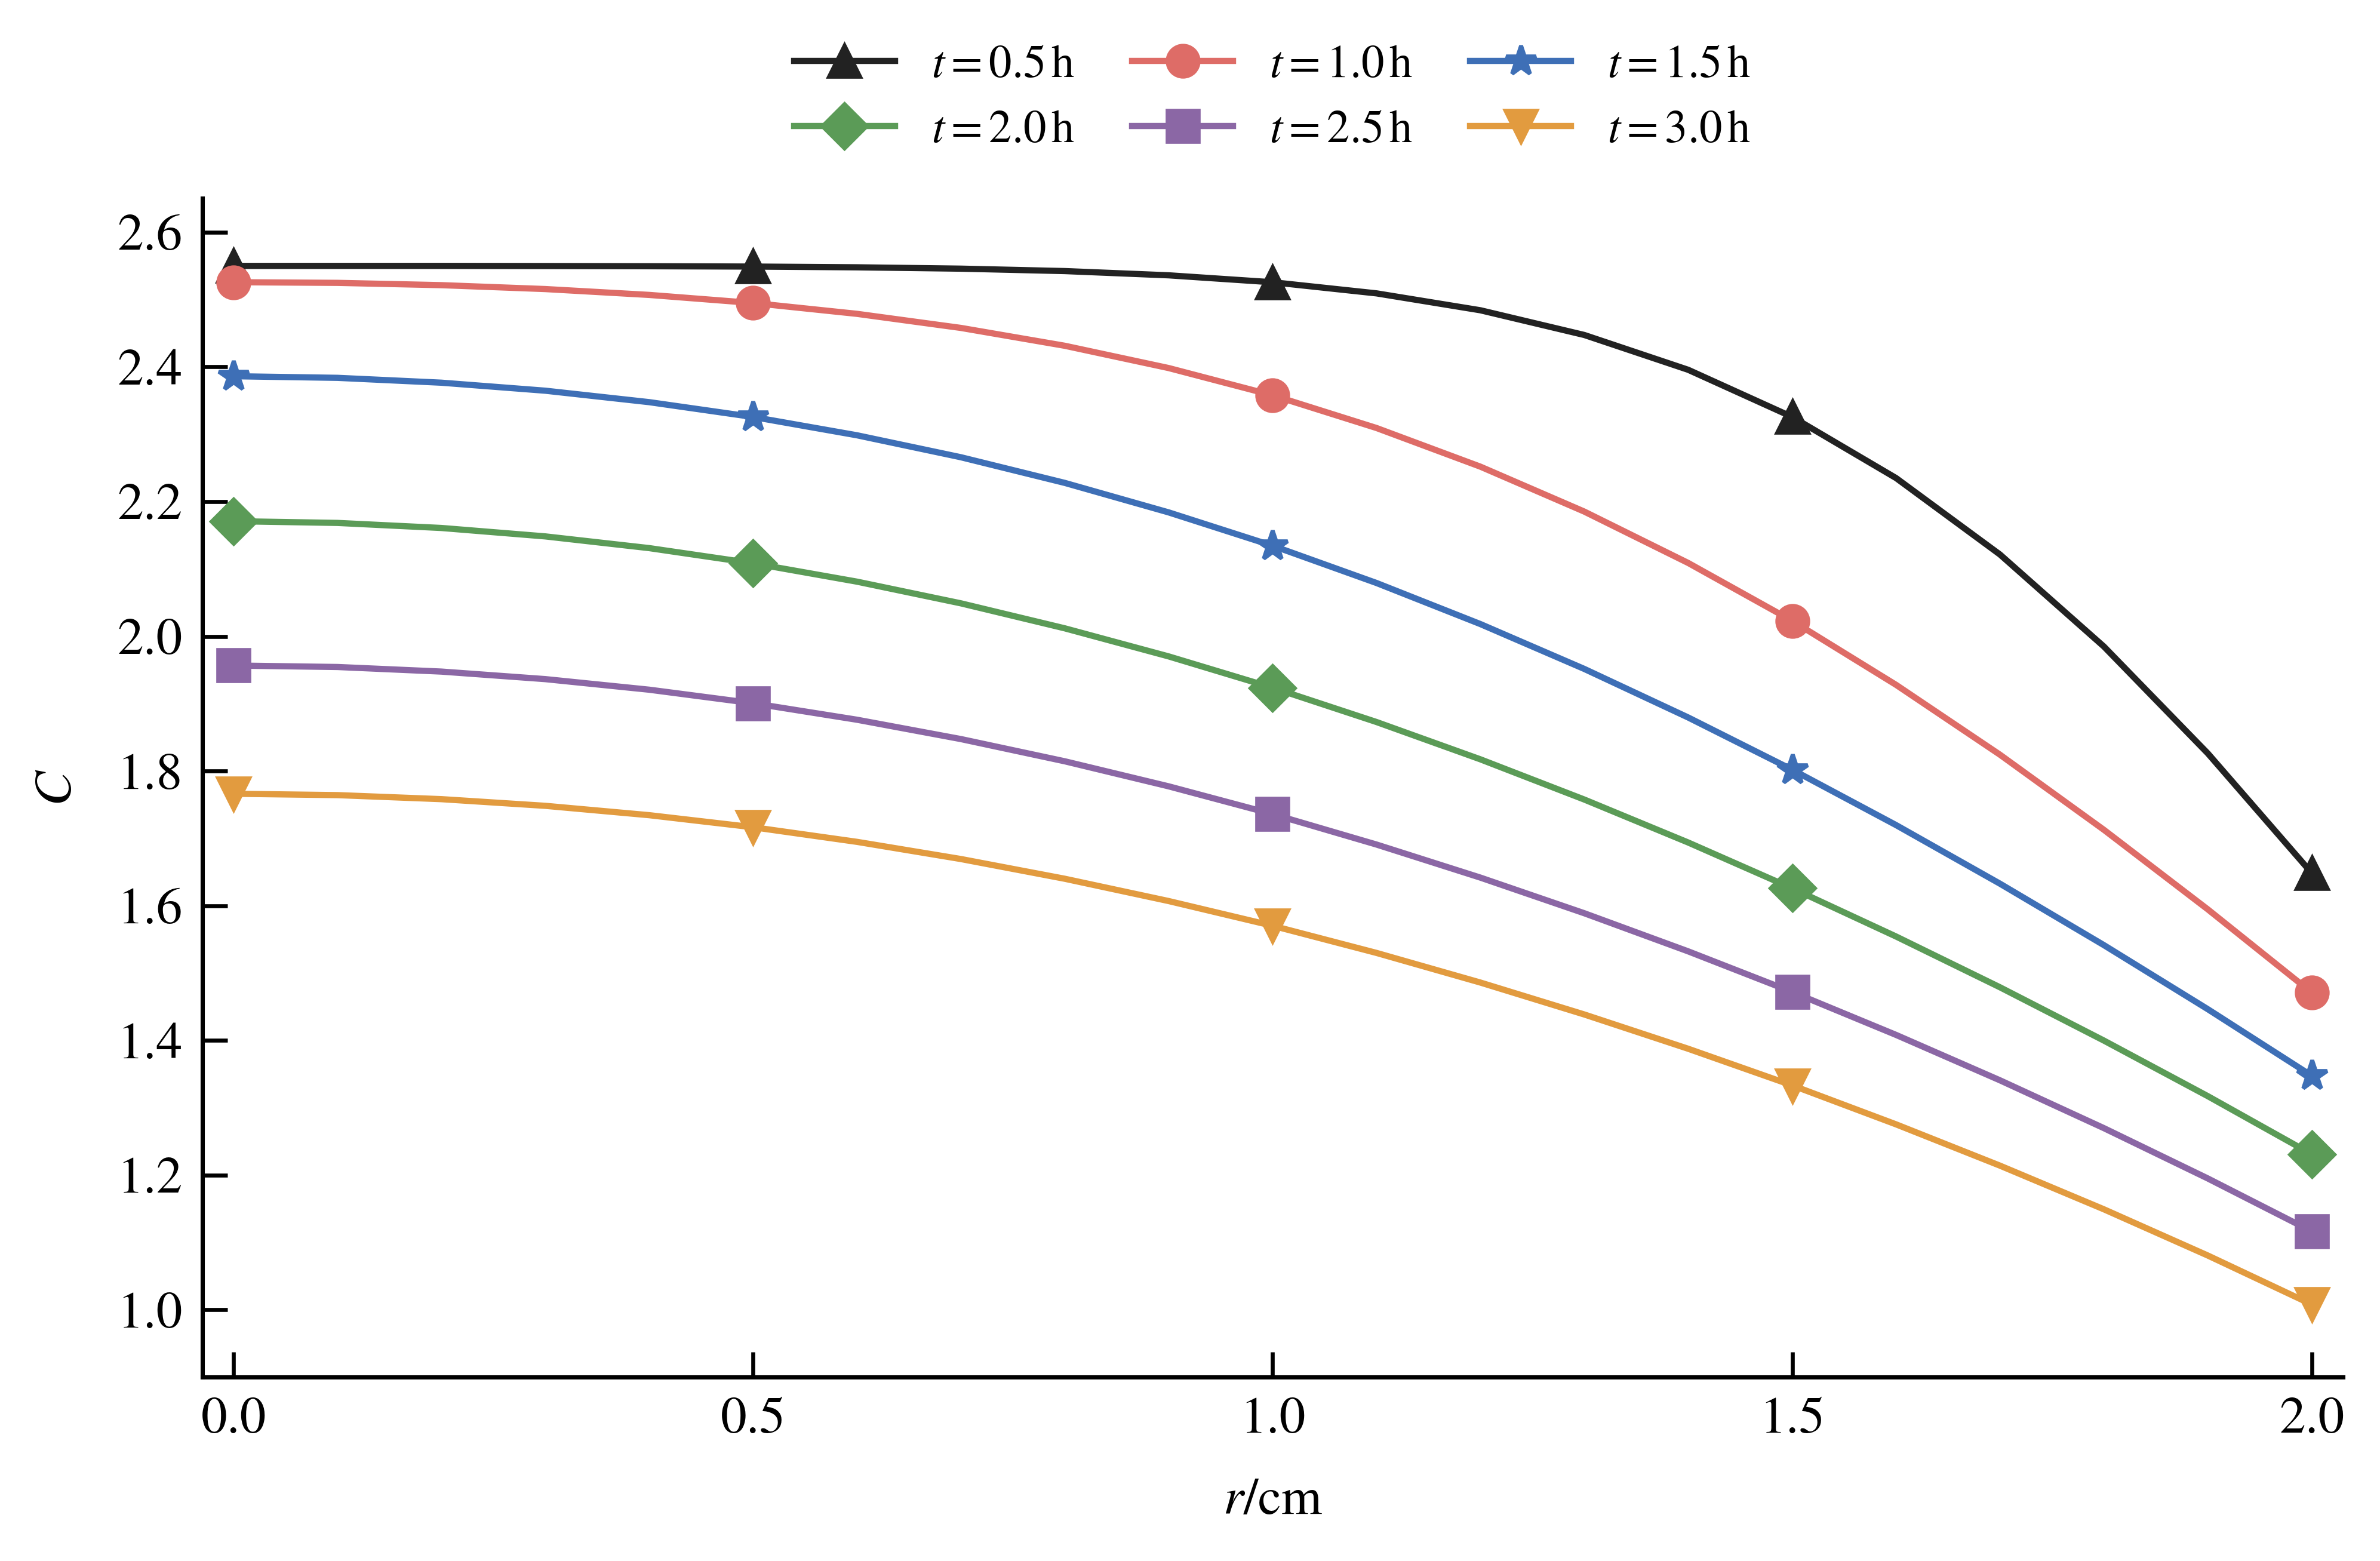
\includegraphics[width=\linewidth]{figures/问题二水分浓度.png}
\caption{水分浓度变化折线图}
\label{fig:q2-moisture-curves}
\end{subfigure}
\caption{问题二模型计算结果}
\label{fig:q2-results}
\end{figure}

\setcounter{table}{3}
\begin{table}[H]
\centering
\renewcommand{\arraystretch}{1.25}
\caption{3小时内药材的温度}
\label{tab:q2-temperature}
\begin{tabularx}{0.9\textwidth}{|>{\centering\arraybackslash}p{0.20\textwidth}|>{\centering\arraybackslash}X|>{\centering\arraybackslash}X|>{\centering\arraybackslash}X|>{\centering\arraybackslash}X|>{\centering\arraybackslash}X|}
\hline
\multirow{2}{*}{时间/h} & \multicolumn{5}{c|}{到药材中心的距离/cm} \\
\cline{2-6}
& 0 & 0.5 & 1 & 1.5 & 2 \\
\hline
0.5 & 32.1892 & 32.3821 & 32.9659 & 33.9608 & 35.4130 \\
\hline
1.0 & 40.3816 & 40.5536 & 41.0605 & 41.8782 & 42.9976 \\
\hline
1.5 & 45.8468 & 45.9348 & 46.1930 & 46.6051 & 47.1401 \\
\hline
2.0 & 48.4502 & 48.4881 & 48.5984 & 48.7736 & 49.0033 \\
\hline
2.5 & 49.4670 & 49.4792 & 49.5136 & 49.5653 & 49.6609 \\
\hline
3.0 & 49.8495 & 49.8553 & 49.8746 & 49.9101 & 49.9664 \\
\hline
\end{tabularx}
\end{table}

\begin{table}[H]
\centering
\renewcommand{\arraystretch}{1.25}
\caption{3小时内药材的水分浓度}
\label{tab:q2-moisture}
\begin{tabularx}{0.9\textwidth}{|>{\centering\arraybackslash}p{0.20\textwidth}|>{\centering\arraybackslash}X|>{\centering\arraybackslash}X|>{\centering\arraybackslash}X|>{\centering\arraybackslash}X|>{\centering\arraybackslash}X|}
\hline
\multirow{2}{*}{时间/h} & \multicolumn{5}{c|}{到药材中心的距离/cm} \\
\cline{2-6}
& 0 & 0.5 & 1 & 1.5 & 2 \\
\hline
0.5 & 2.5499 & 2.5489 & 2.5256 & 2.3257 & 1.6486 \\
\hline
1.0 & 2.5257 & 2.4948 & 2.3578 & 2.0230 & 1.4711 \\
\hline
1.5 & 2.3861 & 2.3256 & 2.1344 & 1.8020 & 1.3476 \\
\hline
2.0 & 2.1709 & 2.1084 & 1.9236 & 1.6259 & 1.2311 \\
\hline
2.5 & 1.9566 & 1.9006 & 1.7360 & 1.4720 & 1.1166 \\
\hline
3.0 & 1.7662 & 1.7165 & 1.5702 & 1.3333 & 1.0081 \\
\hline
\end{tabularx}
\end{table}

\iffalse
% 以下为被删除的旧板凳龙模型正文、结果、模型评价和代码附录，仅保留在源文件中供参考。
{\centering\includegraphics[width=0.715\textwidth]{figures/clip_frag_p24_005.png}\par}

第51 节龙身y (m)

{\centering\includegraphics[width=0.704\textwidth]{figures/clip_frag_p24_006.png}\par}

第101 节龙身x (m)

{\centering\includegraphics[width=0.719\textwidth]{figures/clip_frag_p24_007.png}\par}

第101 节龙身y (m)

{\centering\includegraphics[width=0.709\textwidth]{figures/clip_frag_p24_008.png}\par}

第151 节龙身x (m)

{\centering\includegraphics[width=0.715\textwidth]{figures/clip_frag_p24_009.png}\par}

第151 节龙身y (m)

{\centering\includegraphics[width=0.713\textwidth]{figures/clip_frag_p24_010.png}\par}

第201 节龙身x (m)

{\centering\includegraphics[width=0.715\textwidth]{figures/clip_frag_p24_011.png}\par}

第201 节龙身y (m)

{\centering\includegraphics[width=0.960\textwidth]{figures/clip_frag_p24_012.png}\par}

{\centering\textbf{表6\quad 调头过程中各节龙身速度随时间变化情况}\par}

{\centering\includegraphics[width=0.745\textwidth]{figures/clip_frag_p25_001.png}\par}

{\centering \includegraphics[width=0.451\textwidth]{figures/clip_fig_p25_002.png}\hfill \includegraphics[width=0.451\textwidth]{figures/clip_fig_p25_003.png}\par}

{\centering\includegraphics[width=0.649\textwidth]{figures/clip_frag_p25_004.png}\par}

{\centering \includegraphics[width=0.451\textwidth]{figures/clip_fig_p25_005.png}\hfill \includegraphics[width=0.451\textwidth]{figures/clip_fig_p25_006.png}\par}

{\centering\includegraphics[width=0.654\textwidth]{figures/clip_frag_p25_007.png}\par}

{\centering\textbf{图20\quad 调头过程中不同时刻板凳龙示意图}\par}

\subsubsection{调头运动模型的验证}
使用以上模型求得各时刻每个龙把手的位置与速度后，我们需要简单验证其合理性。

首先，通过使用电脑绘图，可以从视觉上验证位置的正确性。图20是用我们所求坐标绘制的不同时刻板凳龙状态示意图，可以发现板凳龙的把手均按照预定曲线移动，在直观上证实了我们所求坐标的正确性。

其次，我们采用数值微分法，通过选取小时间间隔（如0.01s），计算把手前后位移，再据此计算出平均速度，在时间间隔趋于0 的情况下，该平均速度应收敛于我们使用求导算出的速度。通过与我们利用模型求得的结果对比，可以看出二者之间确实差异较小。利用不同的速度求解方式，我们再一次验证了所求得相关数据的准确性以及所建立模型的合理性。并且相较于直接通过把手位置信息和速度公式求解速度，我们选取的模型能够直接得到更加精确的瞬时速度。

通过对各时刻各节把手的速度分析，我们发现未进入调头空间时，各把手的速度最大值出现在龙头前把手处，这与我们模型一中得出的结论相符。而在龙头前把手进入调头空间后，各把手的速度最大值出现变化。我们发现，在第14s 时，速度最大值出现了短暂的突增。我们猜测是由于龙头开始进入盘出螺线，路径的曲率半径出现较大变化。通过对每时刻舞龙队状态的可视化，我们可以发现在第14s 附近，龙头前把手开始进入曲线N，符合我们的猜想。对速度最大值的分析将会对下一问模型的建立有所帮助。

\subsection{问题五模型建立与求解}
\subsubsection{最大速度计算模型的建立}
题目要求全过程中，所有人的速度不能超过2m/s，求龙头前把手的最大行进速度vmax。注意到在相同位置上，所有把手的速度都成一定比例，也就是说，若龙头的速度从原来的v0 = 1m/s 变为vmax，那么在相同位置上，所有把手的速度都会变为原来的vmax/v0 倍。所以在v0 = 1m/s 时，所有把手速度的最大值一定是

{\centering\includegraphics[width=0.207\textwidth]{figures/clip_frag_p26_001.png}\par}

因此，只要我们借助问题四的模型，求出v0 = 1m/s 时所有把手速度的最大值，就可以算出问题五龙头前把手最大行进速度vmax。

根据要求，本题需要建立一个单目标优化模型，在板凳龙行进的全过程中，最大化速度vn(t)。其中决策变量为时间t。 \textbf{目标函数：}

{\centering\includegraphics[width=0.120\textwidth]{figures/clip_frag_p26_002.png}\par}

\textbf{约束条件：}

$\bullet$ \textbf{时间：}观察问题四得到的各把手的速度数据，不难发现：当t \(\leq\)0 时，

速度的最大值一定出现在龙头，恒为v0；而当t > 0 时，速度的最大值一开始出现

在龙头，后面随着t 的增大，整体呈现向龙尾方向移动的趋势。而且在t = 14s\textasciitilde{}15s

附近（也就是龙头在F 点附近时），速度的最大值突然出现一个极大值。在这之后，

速度的最大值整体呈现缓慢变大的趋势。

因此，我们只需要在龙头在F 点附近和龙尾在F 点附近时计算速度的最大值即可（经计算，该时间间隔为t = 376s\textasciitilde{}384s）。

{\centering\includegraphics[width=0.307\textwidth]{figures/clip_frag_p27_001.png}\par}

因此，我们确定\textbf{所有把手速度最大值的单目标优化模型}为

{\centering\includegraphics[width=0.400\textwidth]{figures/clip_frag_p27_002.png}\par}

\subsubsection{最大速度计算模型的求解}
目标时间范围内t \(\in\)[13s, 16s] \(\cup\)[376s, 384s]，我们以先以0.1s 为步长计算不同时刻下所有把手的最大速度，并比较每个时刻的最大速度。结果表明，所有把手最大速度的最大值出现在t \(\in\)[14s, 15s] 区间内。

通过分析该区间内最大速度的函数变化趋势，我们发现在该时间范围内，把手最大速度的函数图像呈单峰特征，即先增后减。根据此函数性质，我们选用了三分搜索法[2]进一步精确查找在该时间范围内把手的最大速度。

下面是三分搜索法的具体步骤以及示意图：

{\centering \includegraphics[width=0.524\textwidth]{figures/clip_fig_p27_003.png}\par}

{\centering\textbf{图21\quad 三分搜索法示意图}\par}

\textbf{Step 1:} 初始化参数。设定初始搜索区间为[14s, 15s]

\textbf{Step 2:} 计算两个中间点：根据当前区间[left, right]，计算两个三分点：

{\centering\includegraphics[width=0.532\textwidth]{figures/clip_frag_p28_001.png}\par}

分别计算在这两个时间点上的所有把手速度的最大值max

{\centering\includegraphics[width=0.295\textwidth]{figures/clip_frag_p28_002.png}\par}

\textbf{Step 3:} 比较中间点的函数值：• 如果max

{\centering\includegraphics[width=0.925\textwidth]{figures/clip_frag_p28_003.png}\par}

\textbf{Step 4:} 迭代过程：重复步骤2 和步骤3，逐步缩小搜索区间，直到区间的长度小于预设的精度\(\epsilon\) = 10\(-\)8，即|right \(-\)left| < \(\epsilon\)。

\textbf{Step 5:} 求解结果：在最后的迭代结束时，计算最终得到的中点tf = left + right

{\centering\includegraphics[width=0.120\textwidth]{figures/clip_frag_p28_004.png}\par}

应的所有把手速度vn(tf)。根据最小速度限制公式计算龙头前把手的最大速度：

{\centering\includegraphics[width=0.217\textwidth]{figures/clip_frag_p28_005.png}\par}

Step 6: 输出结果：输出最大行进速度vmax，并验证在此速度下所有把手的速度均不超过2m/s。

经计算，我们得出在t \(\approx\)14.47997148s 时，max

{\centering\includegraphics[width=0.463\textwidth]{figures/clip_frag_p28_006.png}\par}

故题目所求结果为vmax \(\approx\)1.246266m/s。

\subsubsection{最大速度优化模型的验证}
通过将所有把手最大速度随时间的变化可视化（图22）后，我们可以发现显然在14s 附近出现了所有把手的最大速度，并且出现在靠近龙头部分。这验证了我们在利用三分法求解速度最大值时选定的时间范围的合理性。

{\centering \includegraphics[width=1.000\textwidth]{figures/clip_fig_p28_007.png}\par}

{\centering\textbf{图22\quad t = \(-\)100s 至t = 500s 把手速度最大值}\par}

{\centering \includegraphics[width=0.623\textwidth]{figures/clip_fig_p29_001.png}\par}

{\centering\textbf{图23\quad t = 14s 至t = 15s 把手速度最大值}\par}

通过画出第14s 至第15s 的所有把手最大速度函数图像（图23，\(\star\)号标注为求得的最大值），我们验证了在该范围区间内使用三分搜索法的合理性，即该函数在给定定义域内仅存在一个极大值，且函数图像呈现先增后减趋势。

\section{模型的评价}
\subsection{模型的优点}
$\bullet$ 模型建立过程中，问题二通过完整证明合理假设，缩小了求解范围，简化了相关模

型；问题四中，对于龙把手不同位置情况进行详细的分类讨论。问题五中，通过巧

妙转化求解目标，同样简化了相关模型。 $\bullet$ 模型求解过程中，通过二分法、粒子群算法、三分搜索法等算法进行优化，并且对

比了不同优化方式的适配与各个模型的适配度，从而选择最优的求解方式，提高求

解效率以及结果的精确度。 $\bullet$ 每个模型都通过不同方式对于最后的求解结果进行验证与分析。

\subsection{模型的缺点}
$\bullet$ 在碰撞检测方法中，并未充分考虑碰撞时物体的物理特性可能会带来的影响。

\section*{参考文献}
{\centering\includegraphics[width=1.000\textwidth]{figures/clip_frag_p30_001.png}\par}
\newpage
{\centering\includegraphics[width=\textwidth]{figures/clip_appendix31_head.png}\par}
\vspace{8pt}
\begin{CodeText}
"""
文件名：dragon.py
用途：第1~3问板凳龙模型(无调头)
"""
import numpy as np
import pandas as pd
import matplotlib.pyplot as plt
from math import *
from matplotlib.font_manager import FontProperties

ben_wid = 0.3 # 板凳宽度(m)
ben_len_head = 3.41 # 龙头板长(m)
ben_len = 2.20 # 龙身及龙尾板长度(m)
hole_dis = 0.275 # 孔离板头距离(m)
hole_dia = 0.055 # 孔的直径(m)
dra_len = 223 # 板凳个数

font = FontProperties(fname="/System/Library/Fonts/Supplemental/Times New Roman.ttf")



font2 = FontProperties(fname="/System/Library/Fonts/Supplemental/Songti.ttc")


class Dragon():

   def __init__(self, d=0.55, v0=1, theta0=32 * pi): # d为螺距(m), v0为龙头前把手速度(m/s)

      self.d = d # 螺距(m)
      self.v0 = v0 # 龙头前把手速度(m/s)
      self.theta0 = theta0 # 0时刻龙头前把手角度

      self.ang = None # 把手角度列表
      self.pos = None # 把手坐标列表
      self.vol = None # 把手速度列表

      self.time = None # 当前时间

   # 设定时间t(s)
   def set_time(self, t, need_vol=False):

      self.time = t # 更新当前时间

      # 求解龙头前把手位置
      theta_n = self.head_pos(t)
      self.ang = [theta_n]
      self.pos = [(self.arc_x(theta_n), self.arc_y(theta_n))]

      if need_vol:
          self.vol = [self.v0]
          d_theta_n = -2 * pi * self.v0 / (self.d * (1 + theta_n**2)**0.5)

      # 求解龙身及龙尾前把手、龙尾后把手位置
      for n in range(223):
          if n != 0:
             theta_n = self.next_pos(theta_n)
          else:
             theta_n = self.next_pos(theta_n, is_head=True)
          self.ang.append(theta_n)
          self.pos.append((self.arc_x(theta_n), self.arc_y(theta_n)))

          if need_vol:
             theta_n0 = self.ang[n]
             theta_n1 = self.ang[n + 1]

             par1 = 2 * theta_n0 - 2 * theta_n1 * cos(theta_n1 - theta_n0) - 2 * theta_n0 *
                       theta_n1 * sin(theta_n1 - theta_n0)
             par2 = 2 * theta_n1 - 2 * theta_n0 * cos(theta_n1 - theta_n0) + 2 * theta_n0 *

                     theta_n1 * sin(theta_n1 - theta_n0)

          d_theta_n1 = -(par1 / par2) * d_theta_n

          v = self.d / (2 * pi) * abs(d_theta_n1) * (1 + theta_n1**2)**0.5
          self.vol.append(v)

          d_theta_n = d_theta_n1

# 判断是否碰撞
def judge_col(self):
   dis_min = 1 # 最短距离(m)

   # 找到距龙头一圈外的第一个板凳
   i_max = 0
   while self.ang[i_max] - self.ang[0] <= 2 * pi:
      i_max += 1

   for i in range(0, i_max + 1):

      l_i = 2.86 if i == 0 else 1.65

      # 找到距第i个板凳一圈外的第一个板凳j0
      j0 = i_max
      while self.ang[j0] - self.ang[i] <= 2 * pi:
          j0 += 1

      # 遍历j0及前后各两个板凳
      # 判断是否相碰
      for j in range(j0 - 2, j0 + 3):
          l_j = 1.65
          delta_xi = self.pos[i + 1][0] - self.pos[i][0]
          delta_yi = self.pos[i + 1][1] - self.pos[i][1]
          delta_xj = self.pos[j + 1][0] - self.pos[j][0]
          delta_yj = self.pos[j + 1][1] - self.pos[j][1]

          s = - delta_yi / l_i # sin(alpha)
          c = - delta_xi / l_i # cos(alpha)

          x1 = self.pos[i][0] + hole_dis * c - (ben_wid / 2) * s
          y1 = self.pos[i][1] + hole_dis * s + (ben_wid / 2) * c
          x2 = self.pos[i + 1][0] - hole_dis * c - (ben_wid / 2) * s
          y2 = self.pos[i + 1][1] - hole_dis * s + (ben_wid / 2) * c

          dis1 = abs(delta_yj * x1 - delta_xj * y1 + self.pos[j + 1][0] * self.pos[j][1] -
                     self.pos[j][0] * self.pos[j + 1][1]) / l_j
          dis2 = abs(delta_yj * x2 - delta_xj * y2 + self.pos[j + 1][0] * self.pos[j][1] -

                      self.pos[j][0] * self.pos[j + 1][1]) / l_j

            if dis1 <= 0.15 or dis2 <= 0.15:
                return True, min(dis1, dis2)

            dis_min = min(dis_min, dis1, dis2)

   return False, dis_min

# 判断龙头前把手到外圈板凳的最短距离
def min_dis(self, t):

   self.set_time(t)
   dis_min = 1 # 最短距离(m)

   # 找到距龙头一圈外的第一个板凳
   j0 = 0
   while self.ang[j0] - self.ang[0] <= 2 * pi:
      j0 += 1

   l_i = 2.86
   for j in range(j0 - 2, j0 + 3):
      l_j = 1.65
      delta_xi = self.pos[1][0] - self.pos[0][0]
      delta_yi = self.pos[1][1] - self.pos[0][1]
      delta_xj = self.pos[j + 1][0] - self.pos[j][0]
      delta_yj = self.pos[j + 1][1] - self.pos[j][1]

      s = - delta_yi / l_i # sin(alpha)
      c = - delta_xi / l_i # cos(alpha)

      x1 = self.pos[0][0] + hole_dis * c - (ben_wid / 2) * s
      y1 = self.pos[0][1] + hole_dis * s + (ben_wid / 2) * c
      x2 = self.pos[1][0] - hole_dis * c - (ben_wid / 2) * s
      y2 = self.pos[1][1] - hole_dis * s + (ben_wid / 2) * c

      dis1 = abs(delta_yj * x1 - delta_xj * y1 + self.pos[j + 1][0] * self.pos[j][1] -
                  self.pos[j][0] * self.pos[j + 1][1]) / l_j
      dis2 = abs(delta_yj * x2 - delta_xj * y2 + self.pos[j + 1][0] * self.pos[j][1] -
                  self.pos[j][0] * self.pos[j + 1][1]) / l_j

      dis_min = min(dis_min, dis1, dis2)

   return dis_min

# 求解相碰时间及此时龙头前把手距中心的距离
def time_col(self):


   time = 0

   # 设定初始状态
   self.set_time(time)

   while not self.judge_col()[0]:
      time += 1
      self.set_time(time)

   return time, self.arc_r(self.ang[0]) # 龙头前把手离中心距离

# 求解龙头前把手到达调头空间的时间
def arr_time(self):
   return binary_search(self.if_arrive, 0, 421, incre=True)

# 打印板凳龙状态(无板凳)
def print_status(self):

   theta = np.linspace(0, 20 * 2 * pi, 1500)
   x = self.d / (2 * pi) * theta * np.cos(theta)
   y = self.d / (2 * pi) * theta * np.sin(theta)

   x_lst = [ben_pos[0] for ben_pos in self.pos]
   y_lst = [ben_pos[1] for ben_pos in self.pos]

   plt.figure()
   plt.plot(x, y, color='black', linewidth=2, alpha=0.5)
   plt.scatter(x_lst, y_lst, color='red', marker='.')

   plt.xlabel('X')
   plt.ylabel('Y')

   plt.grid(True, alpha=0.3)
   plt.show()

# 打印板凳龙图像(有板凳)
def print_img(self, save_pth=None, magn=None, show=True, circle=False):

   # save_pth 保存路径，默认不保存
   # magn 是否放大中心，默认不放大

   a = hole_dis
   b = ben_wid / 2

   # 初始化图像
   plt.figure(figsize=(8, 8))


# 绘制把手
theta = np.linspace(0, 16 * 2 * pi, 1500)
x = self.d / (2 * pi) * theta * np.cos(theta)
y = self.d / (2 * pi) * theta * np.sin(theta)

x_lst = [ben_pos[0] for ben_pos in self.pos]
y_lst = [ben_pos[1] for ben_pos in self.pos]

plt.plot(x, y, color='black', linewidth=2, alpha=0.2)
plt.scatter(x_lst, y_lst, color='red', marker='.')

# 绘制板凳
for i in range(223):

   li = 2.86 if i == 0 else 1.65

   delta_xi = self.pos[i + 1][0] - self.pos[i][0]
   delta_yi = self.pos[i + 1][1] - self.pos[i][1]

   s = - delta_yi / li # sin(alpha)
   c = - delta_xi / li # cos(alpha)

   x1 = self.pos[i][0] + a * c - b * s
   y1 = self.pos[i][1] + a * s + b * c
   x2 = self.pos[i + 1][0] - a * c - b * s
   y2 = self.pos[i + 1][1] - a * s + b * c
   x3 = self.pos[i + 1][0] - a * c + b * s
   y3 = self.pos[i + 1][1] - a * s - b * c
   x4 = self.pos[i][0] + a * c + b * s
   y4 = self.pos[i][1] + a * s - b * c

   rect = [(x1, y1), (x2, y2), (x3, y3), (x4, y4)]

   x, y = zip(*rect)
   plt.plot(x + (x[0],), y + (y[0],), 'b-')

if circle:
   circle = plt.Circle((0, 0), 4.5, color='yellow', fill=True, alpha=0.5)
   plt.gca().add_artist(circle)

# 设置图形属性
plt.xlabel('X', fontproperties=font, size=12)
plt.ylabel('Y', fontproperties=font, size=12)

plt.xticks(fontproperties=font, size=12)
plt.yticks(fontproperties=font, size=12)


   # 放大区域
   if magn is not None:
      plt.xlim(-magn, magn)
      plt.ylim(-magn, magn)

   # 显示图形
   # plt.axis('equal') # 设置坐标轴等比例
   plt.grid(True, alpha=0.3) # 显示网格
   if save_pth:
      plt.savefig(save_pth, dpi=300)
   if show:
      plt.show()
   plt.close()

# (辅助函数）求解龙头前把手角度
def head_pos(self, t):
   par1 = self.theta0 * (1 + self.theta0**2)**0.5
   par2 = log(self.theta0 + (1 + self.theta0**2)**0.5)
   par3 = 4 * pi * self.v0 * t / self.d

   def fn(x):
      return par1 + par2 - par3 - x * (1 + x**2)**0.5 - log(x + (1 + x**2)**0.5)

   return binary_search(fn, 0, self.theta0, incre=False)

# (辅助函数）判断龙头前把手是否进入调头空间
def if_arrive(self, t):
   ang = self.head_pos(t)
   if self.arc_r(ang) <= 4.5:
      return 1
   else:
      return -1

# （辅助函数）求解龙身及龙尾把手角度
def next_pos(self, theta_n, is_head=False): # theta_n为前一把手角度
   l = 2.86 if is_head else 1.65 # 两孔距离(m)
   para1 = (2 * pi * l / self.d)**2

   def fn(x):
      return theta_n**2 + x**2 - 2 * theta_n * x * cos(x - theta_n) - para1

   return binary_search(fn, theta_n, theta_n + pi, incre=True)

# （辅助函数）角度转换为x坐标
def arc_x(self, arc):
   return self.d / (2 * pi) * arc * cos(arc)


   # （辅助函数）角度转换为y坐标
   def arc_y(self, arc):
      return self.d / (2 * pi) * arc * sin(arc)

   # （辅助函数）角度转换为半径
   def arc_r(self, arc):
      return self.d / (2 * pi) * arc


# 二分搜索函数
def binary_search(fn, lb, ub, incre, eps=1e-8):

   cur = (lb + ub) / 2

   while ub - lb > eps:

      cur_res = fn(cur)

      # 若函数递增
      if incre:
            if cur_res < 0:
                lb = cur
            elif cur_res > 0:
                ub = cur

      # 若函数递减
      else:
            if cur_res > 0:
                lb = cur
            elif cur_res < 0:
                ub = cur

      cur = (lb + ub) / 2

   return cur


# 临时测试函数
def test():
   dragon = Dragon()
   dragon.set_time(412)
   dragon.print_img(magn=4)


if __name__ == '__main__':
   test()
\end{CodeText}
\begin{CodeText}
"""
文件名：dragon2.py
用途：第4~5问板凳龙模型(含调头)
"""

"""
请注意
本文档中所有把手角度均为·二元组·
第一个数 表示 所在曲线(1/2/3/4)
第二个数 表示 极角
"""

import numpy as np
import pandas as pd
import matplotlib.pyplot as plt
import matplotlib.patches as patches
from math import *
from matplotlib.font_manager import FontProperties
import os

font = FontProperties(fname="/System/Library/Fonts/Supplemental/Times New Roman.ttf")
font2 = FontProperties(fname="/System/Library/Fonts/Supplemental/Songti.ttc")

ben_wid = 0.3 # 板凳宽度(m)
ben_len_head = 3.41 # 龙头板长(m)
ben_len = 2.20 # 龙身及龙尾板长度(m)
hole_dis = 0.275 # 孔离板头距离(m)
hole_dia = 0.055 # 孔的直径(m)
dra_len = 223 # 板凳个数

d = 1.7 # 螺距(m)
r = 4.5 # 调头空间半径(m)

theta = 2 * pi * r / d # 图中theta角
alpha = atan(theta) # 图中alpha角

R1 = 3 / sin(alpha) # 大圆半径
R2 = 3 / (2 * sin(alpha)) # 小圆半径
# 大圆圆心坐标
O1x = r * cos(theta) - R1 * sin(theta + alpha)
O1y = r * sin(theta) + R1 * cos(theta + alpha)

# 小圆圆心坐标
O2x = -r * cos(theta) + R2 * sin(theta + alpha)

O2y = -r * sin(theta) - R2 * cos(theta + alpha)

# 盘入切点坐标
x1 = d / (2 * pi) * theta * cos(theta)
y1 = d / (2 * pi) * theta * sin(theta)

# 盘出切点坐标
x3 = -x1
y3 = -y1

# 两圆切点坐标
x2 = x1 / 3 + x3 * 2 / 3
y2 = y1 / 3 + y3 * 2 / 3


class Dragon():

   def __init__(self, v0=1): # v0为龙头前把手速度(m/s)

      self.d = d # 螺距(m)
      self.v0 = v0 # 龙头前把手速度(m/s)

      self.ang = None # 把手角度列表
      self.pos = None # 把手坐标列表
      self.vol = None # 把手速度列表

      self.time = None # 当前时间

   # 设定时间t(s)
   def set_time(self, t, need_vol=False):

      self.time = t # 更新当前时间

      # 求解龙头前把手位置
      theta_n = self.head_pos(t)
      self.ang = [theta_n]
      self.pos = [(self.arc_x(theta_n), self.arc_y(theta_n))]

      # 求解龙身及龙尾前把手、龙尾后把手位置
      for n in range(223):
           if n != 0:
              theta_n = self.next_pos(theta_n)
           else:
              theta_n = self.next_pos(theta_n, is_head=True)
           self.ang.append(theta_n)
           self.pos.append((self.arc_x(theta_n), self.arc_y(theta_n)))


# 求解各把手速度
if need_vol == False:
   return

# 求解龙头前把手速度
if self.ang[0][0] == 1:
   d_theta = -2 * pi * self.v0 / d / sqrt(1 + self.ang[0][1] ** 2)
elif self.ang[0][0] == 2:
   d_theta = - self.v0 / R1
elif self.ang[0][0] == 3:
   d_theta = self.v0 / R2
elif self.ang[0][0] == 4:
   d_theta = 2 * pi * self.v0 / d / sqrt(1 + (self.ang[0][1] + pi) ** 2)
self.vol = [self.v0]
d_theta_1 = d_theta

# 求解龙身及龙尾前把手、龙尾后把手速度
for n in range(223):
   l = 2.86 if n == 0 else 1.65
   theta1 = self.ang[n][1]
   theta2 = self.ang[n + 1][1]
   (x1, y1) = self.pos[n]
   (x2, y2) = self.pos[n + 1]

   # 前一把手位于盘入螺线(当前把手位于盘入螺线)
   if self.ang[n][0] == 1:
      par1 = theta1 - theta2 * cos(theta2 - theta1) - theta1 * theta2 * sin(theta2 -
                  theta1)
      par2 = theta2 - theta1 * cos(theta2 - theta1) + theta1 * theta2 * sin(theta2 -
                  theta1)
      d_theta1 = -par1 / par2 * d_theta
      self.vol.append(self.d / (2 * pi) * abs(d_theta1) * sqrt(1 + theta2 ** 2))

   # 前一把手位于大圆圆弧
   elif self.ang[n][0] == 2:

      # 当前把手位于大圆圆弧
      if self.ang[n + 1][0] == 2:
            d_theta1 = d_theta
            self.vol.append(self.vol[n])

      # 当前把手位于盘入螺线
      elif self.ang[n + 1][0] == 1:
            x1d = self.vol[n] * sin(theta1)
            y1d = -self.vol[n] * cos(theta1)
            par1 = (x1 - d / (2 * pi) * theta2 * cos(theta2)) * x1d + (y1 - d / (2 * pi)
                      * theta2 * sin(theta2)) * y1d

      par2 = (x1 - d / (2 * pi) * theta2 * cos(theta2)) * (cos(theta2) - theta2 *
                 sin(theta2)) + (y1 - d / (2 * pi) * theta2 * sin(theta2)) * (sin(theta2)
                 + theta2 * cos(theta2))
      d_theta1 = 2 * pi / d * par1 / par2
      self.vol.append(self.d / (2 * pi) * abs(d_theta1) * sqrt(1 + theta2 ** 2))

# 前一把手位于小圆圆弧
elif self.ang[n][0] == 3:

   # 当前把手位于小圆圆弧
   if self.ang[n + 1][0] == 3:
      d_theta1 = d_theta
      self.vol.append(self.vol[n])

   # 当前把手位于大圆圆弧
   elif self.ang[n + 1][0] == 2:
      x1d = self.vol[n] * sin(theta1)
      y1d = -self.vol[n] * cos(theta1)
      par1 = (x1 - O1x - R1 * cos(theta2)) * x1d + (y1 - O1y - R1 * sin(theta2)) *
                 y1d
      par2 = (x1 - O1x - R1 * cos(theta2)) * sin(theta2) - (y1 - O1y - R1 *
                 sin(theta2)) * cos(theta2)
      d_theta1 = -par1 / (R1 * par2)
      self.vol.append(abs(d_theta1) * R1)

# 前一把手位于盘出螺线
elif self.ang[n][0] == 4:

   # 当前把手位于盘出螺线
   if self.ang[n + 1][0] == 4:
      theta1, theta2 = theta1 + pi, theta2 + pi
      par1 = theta1 - theta2 * cos(theta2 - theta1) - theta1 * theta2 * sin(theta2
                 - theta1)
      par2 = theta2 - theta1 * cos(theta2 - theta1) + theta1 * theta2 * sin(theta2
                 - theta1)
      d_theta1 = -par1 / par2 * d_theta
      self.vol.append(self.d / (2 * pi) * abs(d_theta1) * sqrt(1 + theta2 ** 2))
      theta1, theta2 = theta1 - pi, theta2 - pi

   # 当前把手位于小圆圆弧
   elif self.ang[n + 1][0] == 3:
      beta = theta1 + atan(theta1 + pi)
      x1d = self.vol[n] * cos(beta)
      y1d = self.vol[n] * sin(beta)
      par1 = (x1 - O2x + R2 * cos(theta2)) * x1d + (y1 - O2y + R2 * sin(theta2)) *
                 y1d
      par2 = (x1 - O2x + R2 * cos(theta2)) * sin(theta2) - (y1 - O2y + R2 *

                          sin(theta2)) * cos(theta2)
                d_theta1 = par1 / (R2 * par2)
                self.vol.append(abs(d_theta1) * R2)

      d_theta = d_theta1

# 打印板凳龙状态(无板凳)
def print_status(self):

   # 计算盘入盘出螺线
   ang = np.linspace(theta, 10 * 2 * pi, 1000)
   xx1 = d / (2 * pi) * ang * np.cos(ang)
   yy1 = d / (2 * pi) * ang * np.sin(ang)
   xx2 = -xx1
   yy2 = -yy1

   plt.figure(figsize=(8, 8))

   # 绘制盘入盘出螺线
   plt.plot(xx1, yy1, color='red', linewidth=2, label='盘入螺线', alpha=0.5)
   plt.plot(xx2, yy2, color='blue', linewidth=2, label='盘出螺线', alpha=0.5)
   plt.plot([], [], color='black', linewidth=2, label='调头路径', alpha=0.5)

   # 绘制调头空间
   circle = plt.Circle((0, 0), 4.5, color='yellow', fill=True, alpha=0.4)
   plt.gca().add_artist(circle)

   # 绘制两圆圆心
   # plt.scatter(O1x, O1y, color='black', marker='.', alpha=0.5)
   # plt.scatter(O2x, O2y, color='black', marker='.', alpha=0.5)

   # 绘制调头路径
   arc1 = patches.Arc((O1x, O1y), width=R1 * 2, height=R1 * 2, theta1=np.rad2deg(theta -
             alpha - pi / 2), theta2=np.rad2deg(theta + alpha - pi / 2), color='black',
             linewidth=2, alpha=0.5)
   plt.gca().add_patch(arc1)

   arc2 = patches.Arc((O2x, O2y), width=R2 * 2, height=R2 * 2, theta1=np.rad2deg(theta -
             alpha + pi / 2), theta2=np.rad2deg(theta + alpha + pi / 2), color='black',
             linewidth=2, alpha=0.5)
   plt.gca().add_patch(arc2)

   x_lst = [ben_pos[0] for ben_pos in self.pos]
   y_lst = [ben_pos[1] for ben_pos in self.pos]

   plt.scatter(x_lst, y_lst, color='black', marker='.')


   plt.axis('equal')
   plt.xlabel('X', fontproperties=font, size=12)
   plt.ylabel('Y', fontproperties=font, size=12)
   plt.xticks(fontproperties=font, size=12)
   plt.yticks(fontproperties=font, size=12)

   plt.grid(True, alpha=0.3)
   plt.show()

# 打印板凳龙图像(有板凳)
def print_img(self, save_pth=None, magn=None, show=True):

   # save_pth 保存路径，默认不保存
   # magn 是否放大中心，默认不放大
   # show 是否展示，默认展示

   # 初始化图像
   plt.figure(figsize=(8, 8))

   # 计算盘入盘出螺线
   ang = np.linspace(theta, 10 * 2 * pi, 1000)
   xx1 = d / (2 * pi) * ang * np.cos(ang)
   yy1 = d / (2 * pi) * ang * np.sin(ang)
   xx2 = -xx1
   yy2 = -yy1

   # 绘制盘入盘出螺线
   plt.plot(xx1, yy1, color='red', linewidth=2, label='盘入螺线', alpha=0.5)
   plt.plot(xx2, yy2, color='blue', linewidth=2, label='盘出螺线', alpha=0.5)
   plt.plot([], [], color='black', linewidth=2, label='调头路径', alpha=0.5)

   # 绘制调头空间
   circle = plt.Circle((0, 0), 4.5, color='yellow', fill=True, alpha=0.4)
   plt.gca().add_artist(circle)

   # 绘制两圆圆心
   # plt.scatter(O1x, O1y, color='black', marker='.', alpha=0.5)
   # plt.scatter(O2x, O2y, color='black', marker='.', alpha=0.5)

   # 绘制调头路径
   arc1 = patches.Arc((O1x, O1y), width=R1 * 2, height=R1 * 2, theta1=np.rad2deg(theta -
             alpha - pi / 2), theta2=np.rad2deg(theta + alpha - pi / 2), color='black',
             linewidth=2, alpha=0.5)
   plt.gca().add_patch(arc1)

   arc2 = patches.Arc((O2x, O2y), width=R2 * 2, height=R2 * 2, theta1=np.rad2deg(theta -
             alpha + pi / 2), theta2=np.rad2deg(theta + alpha + pi / 2), color='black',

          linewidth=2, alpha=0.5)
plt.gca().add_patch(arc2)

# 绘制把手
x_lst = [ben_pos[0] for ben_pos in self.pos]
y_lst = [ben_pos[1] for ben_pos in self.pos]

plt.scatter(x_lst, y_lst, color='black', marker='.')

# 绘制板凳
a = hole_dis
b = ben_wid / 2

for i in range(223):

   li = 2.86 if i == 0 else 1.65

   delta_xi = self.pos[i + 1][0] - self.pos[i][0]
   delta_yi = self.pos[i + 1][1] - self.pos[i][1]

   s = - delta_yi / li # sin(alpha)
   c = - delta_xi / li # cos(alpha)

   x1 = self.pos[i][0] + a * c - b * s
   y1 = self.pos[i][1] + a * s + b * c
   x2 = self.pos[i + 1][0] - a * c - b * s
   y2 = self.pos[i + 1][1] - a * s + b * c
   x3 = self.pos[i + 1][0] - a * c + b * s
   y3 = self.pos[i + 1][1] - a * s - b * c
   x4 = self.pos[i][0] + a * c + b * s
   y4 = self.pos[i][1] + a * s - b * c

   rect = [(x1, y1), (x2, y2), (x3, y3), (x4, y4)]

   x, y = zip(*rect)
   plt.plot(x + (x[0],), y + (y[0],), 'b-')

# 设置图形属性
plt.xlabel('X', fontproperties=font, size=12)
plt.ylabel('Y', fontproperties=font, size=12)

plt.xticks(fontproperties=font, size=12)
plt.yticks(fontproperties=font, size=12)

# 放大区域
if magn is not None:
   plt.xlim(-magn, magn)

      plt.ylim(-magn, magn)

   # 显示图形
   # plt.axis('equal') # 设置坐标轴等比例
   plt.grid(True, alpha=0.3)
   if save_pth:
      plt.savefig(save_pth, dpi=300)
   if show:
      plt.show()
   plt.close()

# 保存板凳龙图像
def save_imgs(self, start_t, end_t, save_pth="photos2", magn=8):
   for time in np.arange(start_t, end_t + 1, 1):
      print("time = ", time)
      self.set_time(time)
      self.print_img(os.path.join(save_pth, f"{time}.png"), magn=magn, show=False)

# (辅助函数）求解龙头前把手角度
def head_pos(self, t):

   # 位于盘入螺线
   if t <= 0:
      par1 = theta * (1 + theta**2)**0.5
      par2 = log(theta + (1 + theta**2)**0.5)
      par3 = 4 * pi * self.v0 * t / self.d

      def fn(x):
           return par1 + par2 - par3 - x * (1 + x**2)**0.5 - np.log(x + (1 + x**2)**0.5)

      return 1, binary_search(fn, theta, theta * 2, incre=False)

   # 位于大圆圆弧
   elif t < 6 * alpha / (sin(alpha) * self.v0):
      theta_n = theta + alpha - pi / 2 - self.v0 * t / R1
      return 2, theta_n

   # 位于小圆圆弧
   elif t < 9 * alpha / (sin(alpha) * self.v0):
      theta_n = theta - alpha - pi / 2 + self.v0 * (t - 2 * alpha * R1 / self.v0) / R2
      return 3, theta_n

   # 位于盘出螺线
   else:
      par1 = theta * (1 + theta**2)**0.5
      par2 = log(theta + (1 + theta**2)**0.5)
      par3 = 4 * pi * self.v0 * (t - 2 * alpha * (R1 + R2) / self.v0) / self.d


      def fn(x):
            return x * (1 + x**2)**0.5 + np.log(x + (1 + x**2)**0.5) - par1 - par2 - par3

      return 4, binary_search(fn, theta, theta * 20, incre=True) - pi

# （辅助函数）龙头前把手路径图
def head_img(self):

   # 计算盘入盘出螺线
   ang = np.linspace(theta, 6 * 2 * pi, 1000)
   x1 = d / (2 * pi) * ang * np.cos(ang)
   y1 = d / (2 * pi) * ang * np.sin(ang)
   x2 = -x1
   y2 = -y1

   plt.figure(figsize=(8, 8))

   # 绘制盘入盘出螺线
   plt.plot(x1, y1, color='red', linewidth=2, label='盘入螺线', alpha=0.5)
   plt.plot(x2, y2, color='blue', linewidth=2, label='盘出螺线', alpha=0.5)
   plt.plot([], [], color='black', linewidth=2, label='调头路径', alpha=0.5)

   # 绘制调头空间
   circle = plt.Circle((0, 0), 4.5, color='yellow', fill=True, alpha=0.4)
   plt.gca().add_artist(circle)

   # 绘制两圆圆心
   plt.scatter(O1x, O1y, color='black', marker='.', alpha=0.5)
   plt.scatter(O2x, O2y, color='black', marker='.', alpha=0.5)

   # 绘制调头路径
   arc1 = patches.Arc((O1x, O1y), width=R1 * 2, height=R1 * 2, theta1=np.rad2deg(theta -
             alpha - pi / 2), theta2=np.rad2deg(theta + alpha - pi / 2), color='black',
             linewidth=2, alpha=0.5)
   plt.gca().add_patch(arc1)

   arc2 = patches.Arc((O2x, O2y), width=R2 * 2, height=R2 * 2, theta1=np.rad2deg(theta -
             alpha + pi / 2), theta2=np.rad2deg(theta + alpha + pi / 2), color='black',
             linewidth=2, alpha=0.5)
   plt.gca().add_patch(arc2)

   x = []
   y = []

   for t in np.arange(-100, 101):
      ang = self.head_pos(t)

      x.append(self.arc_x(ang))
      y.append(self.arc_y(ang))

   plt.scatter(x, y, marker='*', color='black')

   plt.axis('equal')
   plt.xlabel('X', fontproperties=font, size=12)
   plt.ylabel('Y', fontproperties=font, size=12)
   plt.xticks(fontproperties=font, size=12)
   plt.yticks(fontproperties=font, size=12)

   plt.legend(prop=font2)
   plt.grid(True, alpha=0.2)
   # plt.savefig("Figure_8.png")
   plt.show()

# （辅助函数）求解龙身及龙尾把手角度
def next_pos(self, theta_n, is_head=False): # theta_n为前一把手角度

   l = 2.86 if is_head else 1.65 # 两孔距离(m)

   # 前一把手位于盘入螺线（当前把手位于盘入螺线）
   if theta_n[0] == 1:
      theta_n = theta_n[1]
      par1 = (2 * pi * l / self.d)**2

      def fn(x):
         return theta_n**2 + x**2 - 2 * theta_n * x * cos(x - theta_n) - par1

      return 1, binary_search(fn, theta_n, theta_n + pi, incre=True)

   # 前一把手位于大圆圆弧
   elif theta_n[0] == 2:
      xn = self.arc_x(theta_n)
      yn = self.arc_y(theta_n)

      # 当前把手位于盘入螺线
      if dist((xn, yn), (x1, y1)) <= l:

         def fn(x):
                par1 = d / (2 * pi) * x * np.cos(x)
                par2 = d / (2 * pi) * x * np.sin(x)
                return (xn - par1)**2 + (yn - par2)**2 - l**2

         return 1, binary_search(fn, theta_n[1], theta_n[1] + pi, incre=True)

      # 当前把手位于大圆圆弧

   else:
      delta_theta = 2 * asin(l / (2 * R1))
      return 2, theta_n[1] + delta_theta

# 前一把手位于小圆圆弧
elif theta_n[0] == 3:
   xn = self.arc_x(theta_n)
   yn = self.arc_y(theta_n)

   # 当前把手位于大圆圆弧
   if dist((xn, yn), (x2, y2)) <= l:

      def fn(x):
           par1 = xn - O1x - R1 * np.cos(x)
           par2 = yn - O1y - R1 * np.sin(x)
           return par1**2 + par2**2 - l**2

      return 2, binary_search(fn, theta - alpha - pi / 2, theta + alpha - pi / 2,
                 incre=True)

   # 当前把手位于小圆圆弧
   else:
      delta_theta = 2 * asin(l / (2 * R2))
      return 3, theta_n[1] - delta_theta

# 前一把手位于盘出螺线
elif theta_n[0] == 4:
   xn = self.arc_x(theta_n)
   yn = self.arc_y(theta_n)

   # 当前把手位于小圆圆弧
   if dist((xn, yn), (x3, y3)) <= l and theta_n[1] <= theta:

      def fn(x):
           par1 = xn - O2x + R2 * np.cos(x)
           par2 = yn - O2y + R2 * np.sin(x)
           return par1**2 + par2**2 - l**2

      return 3, binary_search(fn, theta - alpha - pi / 2, theta + alpha - pi / 2,
                 incre=False)

   # 当前把手位于盘出螺线
   else:
      theta_n = theta_n[1]
      par1 = (2 * pi * l / self.d)**2

      def fn(x):

                 return (theta_n + pi)**2 + (x + pi)**2 - 2 * (theta_n + pi) * (x + pi) *
                           cos(x - theta_n) - par1

             return 4, binary_search(fn, theta_n - pi, theta_n, incre=False)

   # （辅助函数）角度转换为x坐标
   def arc_x(self, arc):

      # 位于盘入螺线
      if arc[0] == 1:
          return self.d / (2 * pi) * arc[1] * cos(arc[1])

      # 位于大圆圆弧
      elif arc[0] == 2:
          return O1x + R1 * cos(arc[1])

      # 位于小圆圆弧
      elif arc[0] == 3:
          return O2x - R2 * cos(arc[1])

      # 位于盘出螺线
      elif arc[0] == 4:
          return self.d / (2 * pi) * (arc[1] + pi) * cos(arc[1])

   # （辅助函数）角度转换为y坐标
   def arc_y(self, arc):

      # 位于盘入螺线
      if arc[0] == 1:
          return self.d / (2 * pi) * arc[1] * sin(arc[1])

      # 位于大圆圆弧
      elif arc[0] == 2:
          return O1y + R1 * sin(arc[1])

      # 位于小圆圆弧
      elif arc[0] == 3:
          return O2y - R2 * sin(arc[1])

      # 位于盘出螺线
      elif arc[0] == 4:
          return self.d / (2 * pi) * (arc[1] + pi) * sin(arc[1])


# 二分搜索函数
def binary_search(fn, lb, ub, incre, eps=1e-8):


      cur = (lb + ub) / 2

      while ub - lb > eps:

         cur_res = fn(cur)

         # 若函数递增
         if incre:
               if cur_res < 0:
                   lb = cur
               elif cur_res > 0:
                   ub = cur

         # 若函数递减
         else:
               if cur_res > 0:
                   lb = cur
               elif cur_res < 0:
                   ub = cur

         cur = (lb + ub) / 2

      return cur

# 求两点间距离
def dist(p1, p2):
      return ((p1[0] - p2[0])**2 + (p1[1] - p2[1])**2)**0.5


# 临时测试函数
def test():
      dragon = Dragon()
      dragon.set_time(300)
      dragon.print_img(magn=8)


if __name__ == '__main__':
      test()
\end{CodeText}
\begin{CodeText}
"""
文件名：problem1_1.py
用途：求解0~300s各把手位置
"""
from dragon import *

col_0 = ['龙头x (m)', '龙头y (m)']

for i in range(1, 222):
      col_0.append(f'第{i}节龙身x (m)')
      col_0.append(f'第{i}节龙身y (m)')
col_0.extend(['龙尾x (m)', '龙尾y (m)', '龙尾（后）x (m)', '龙尾（后）y (m)'])

data = {'': col_0}

dragon = Dragon()

for time in range(301):

      if time % 10 == 0:
         print(f"已求解{time}s")

      dragon.set_time(time)

      xy_lst = []
      for x, y in dragon.pos:
         xy_lst.append(x)
         xy_lst.append(y)

      data[f'{time} s'] = xy_lst

df = pd.DataFrame(data)
df.to_csv('result1_pos.csv', index=False)
\end{CodeText}
\begin{CodeText}
"""
文件名：problem1_2.py
用途：求解0~300s各把手速度
"""
from dragon import *

col_0 = ['龙头 (m/s)']
for i in range(1, 222):
      col_0.append(f'第{i}节龙身 (m/s)')
col_0.extend(['龙尾 (m/s)', '龙尾（后） (m/s)'])

data = {'': col_0}

dragon = Dragon()

for time in range(301):

      if time % 10 == 0:
         print(f"已求解{time}s")


      dragon.set_time(time, need_vol=True)

      data[f'{time} s'] = dragon.vol

df = pd.DataFrame(data)
df.to_csv('result1_vol.csv', index=False)
\end{CodeText}
\begin{CodeText}
"""
文件名：problem2_1.py
用途：变步长求解碰撞时刻
"""
from dragon import *

dragon = Dragon()

def check_col(start, end, step):
      for time in np.arange(start, end, step):
         dragon.set_time(time)
         coll = dragon.judge_col()
         print("time = ", time, " if_collision = ", coll[0], " min_dis = ", coll[1])

check_col(412, 413, 0.1)
\end{CodeText}
\begin{CodeText}
"""
文件名：problem2_2.py
用途：求解碰撞时刻各把手的位置和速度
"""
from dragon import *

col_time = 412.47383777 # 碰撞时刻(s)

dragon = Dragon()
dragon.set_time(col_time, need_vol=True)

col_0 = ['龙头']
for i in range(1, 222):
      col_0.append(f'第{i}节龙身')
col_0.extend(['龙尾', '龙尾（后）'])

data = {'': col_0}

data['横坐标x (m)'] = [ben_pos[0] for ben_pos in dragon.pos]
data['纵坐标y (m)'] = [ben_pos[1] for ben_pos in dragon.pos]
data['速度 (m/s)'] = dragon.vol

df = pd.DataFrame(data)

df.to_csv('result2_all.csv', index=False)
\end{CodeText}
\begin{CodeText}
"""
文件名：problem3.py
用途：求解龙头前把手能进入调头空间的最小螺距
"""
from dragon import *
from sko.PSO import PSO


def min_pitch(start, end, step, fig1=False, fig2=False):

      for d in np.arange(start, end, step):
         dragon = Dragon(d=d)
         time = dragon.arr_time()
         print(f'当前螺距为{d}m')

         pso = PSO(func=dragon.min_dis, n_dim=1, pop=40, max_iter=50, lb=0, ub=time, w=0.8,
                  c1=0.5, c2=0.5)
         pso.run()
         dist = pso.gbest_y
         print('best_x is ', pso.gbest_x, 'best_y is', pso.gbest_y)

         # 作图1
         if fig1:
            xx = np.linspace(0, time, 1000)
            yy = np.array([dragon.min_dis(x) for x in xx])
            plt.figure()
            plt.plot(xx, yy)
            plt.plot(pso.gbest_x, pso.gbest_y, '*r')
            plt.xlabel('时间t(s)', fontproperties=font2, size=12)
            plt.ylabel('A点和B点距其他板凳中心线的最短距离', fontproperties=font2, size=12)
            plt.xticks(fontproperties=font, size=12)
            plt.yticks(fontproperties=font, size=12)
            plt.savefig("Figure_4.png", dpi=300)
            plt.show()

         # 作图2
         if fig2:
            plt.figure(figsize=(7, 5))
            plt.plot(pso.gbest_y_hist)
            plt.xlabel('粒子群迭代次数', fontproperties=font2, size=12)
            plt.ylabel('全局最优解的函数值', fontproperties=font2, size=12)
            plt.xticks(fontproperties=font, size=12)
            plt.yticks(fontproperties=font, size=12)
            plt.savefig("Figure_6.png", dpi=300)

            plt.show()

         if dist > 0.15:
            break


if __name__ == '__main__':
      min_pitch(0.45, 0.46, 0.001)
\end{CodeText}
\begin{CodeText}
"""
文件名：problem4_1.py
用途：求解-100~100s各把手的位置
"""
from dragon2 import *

col_0 = ['龙头x (m)', '龙头y (m)']
for i in range(1, 222):
      col_0.append(f'第{i}节龙身x (m)')
      col_0.append(f'第{i}节龙身y (m)')
col_0.extend(['龙尾x (m)', '龙尾y (m)', '龙尾（后）x (m)', '龙尾（后）y (m)'])

data = {'': col_0}

dragon = Dragon()
for time in np.arange(-100, 101, 1):

      if time % 10 == 0:
         print(f"已求解到{time}s")

      dragon.set_time(time)
      xy_lst = []
      for x, y in dragon.pos:
         xy_lst.append(x)
         xy_lst.append(y)

      data[f"{time} s"] = xy_lst

df = pd.DataFrame(data)
df.to_csv('result4_pos.csv', index=False)
\end{CodeText}
\begin{CodeText}
"""
文件名：problem4_2.py
用途：求解-100~100s各把手的速度
"""
from dragon2 import *


col_0 = ['龙头 (m/s)']
for i in range(1, 222):
      col_0.append(f'第{i}节龙身 (m/s)')
col_0.extend(['龙尾 (m/s)', '龙尾（后） (m/s)'])

data = {'': col_0}

dragon = Dragon()
for time in np.arange(-100, 101, 1):

      if time % 10 == 0:
         print(f"已求解到{time}s")

      dragon.set_time(time, need_vol=True)

      data[f"{time} s"] = dragon.vol

df = pd.DataFrame(data)
df.to_csv('result4_vol.csv', index=False)
\end{CodeText}
\begin{CodeText}
"""
文件名：problem5.py
用途：求解全局把手最大速度
"""
from dragon2 import *

dragon = Dragon()


# 求某时刻的最大速度
def max_vt(time):
      dragon.set_time(time, need_vol=True)
      return max(dragon.vol)


# 求某时间段内的最大速度
def max_v(start, end, step, save_pth=None):

      glo_max_v = 0 # 全局最大速度
      max_time = 0 # 最大速度对应时间

      for time in np.arange(start, end, step):
         dragon.set_time(time, need_vol=True)
         cur_max_v = max(dragon.vol)

         if cur_max_v > glo_max_v:

          glo_max_v = cur_max_v
          max_time = time

      print("time = ", time, " max_v = ", cur_max_v)

   print(glo_max_v, max_time)

   plt.figure(figsize=(20, 7))

   xx = np.arange(start, end, step)
   yy = [max_vt(x) for x in xx]
   plt.plot(xx, yy, color='#00C5D7', linewidth=2)

   plt.xlabel('时间t(s)', fontproperties=font2, size=12)
   plt.ylabel('把手最大速度(m/s)', fontproperties=font2, size=12)
   plt.xticks(fontproperties=font, size=12)
   plt.yticks(fontproperties=font, size=12)

   plt.grid(True, alpha=0.3)
   if save_pth:
      plt.savefig(save_pth, dpi=300)
   plt.show()


# 三分搜索算法(求极大值)
def ternary_search(fn, lb, ub, eps=1e-8):

   while ub - lb >= eps:

      margin = (ub - lb) / 3
      x1 = lb + margin
      x2 = ub - margin

      if fn(x1) <= fn(x2):
          lb = x1
      else:
          ub = x2

   return (lb + ub) / 2


# 三分搜索法求最大速度
def main(save_pth=None, show=True):

   t = ternary_search(max_vt, 14, 15)
   f_t = max_vt(t)


   print(t, f_t)

   if show:
      plt.figure()

      xx = np.arange(14, 15, 0.01)
      yy = [max_vt(x) for x in xx]
      plt.plot(xx, yy, color='#00A7E3', linewidth=2)

      plt.plot(t, f_t, marker='*', color='red')

      plt.xlabel('时间t(s)', fontproperties=font2, size=12)
      plt.ylabel('把手最大速度(m/s)', fontproperties=font2, size=12)
      plt.xticks(fontproperties=font, size=12)
      plt.yticks(fontproperties=font, size=12)

      plt.grid(True, alpha=0.3)
      if save_pth is not None:
          plt.savefig(save_pth, dpi=300)
      plt.show()


if __name__ == '__main__':
   main(save_pth="Figure_10.png")
\end{CodeText}
\fi
\end{document}
